\section{Generating Code for Patterns}

\subsection{Introduction}

\begin{enumerate}
\item
`isa` procedure that accepts a term and decides (true/false) if it matches desired pattern. This is done by ensuring each term instance is of expected class (e.g. \texttt{Integer}) and additionally verifying side conditions (e.g. \texttt{natural} term must of class \texttt{Integer} and its value must be greater or equal to zero)
\item
Actual matching procedure that accepts a match object, a term, and two extra arguments `head` and `tail` which indicate a range of subterms in the term that haven't been matched yet. Successful matching increments value of \texttt{head} by one. In principle it should be possible to perform pattern matching bi-directionally but PyPltRedex doesn't implement this.
\item
Top-level matching procedure that accepts a term, initializes `Match` object with pattern-variables found in the pattern and calls matching procedure. `Match` objects filtered and returned.
\end{enumerate}


\subsection{Is-A Procedures}

So called Is-A procedures have the following interface:

\begin{lstlisting}
isa(term: Term) -> boolean
\end{lstlisting}

These procedures are produced for all built-in patterns excluding `(inhole pattern pattern)`.  Originally, most these procedures were generated by PyPltRedex dynamically but then I realized these could just a part of runtime library introduced in Chapter TODO. This allowed for great code generator simplification.

\begin{lstlisting}
def term_is_number(term):
    return isinstance(term, Float) or isinstance(term, Integer)

def term_is_integer(term):
    return isinstance(term, Integer) 

def term_is_float(term):
    return isinstance(term, Float) 

def term_is_natural_number(term):
    return isinstance(term, Integer) and term.value() >= 0

def term_is_hole(term):
    return isinstance(term, Hole) 

def term_is_string(term):
    return isinstance(term, String) 

def term_is_boolean(term):
    return isinstance(term, Boolean) 

def term_is_variable_not_otherwise_mentioned(term, variableset):
    return isinstance(term, Variable) and term.value() not in variableset
\end{lstlisting}

Figure above demonstrates \texttt{isa} procedures for \texttt{number}, \texttt{real}, \texttt{natural}, \texttt{string}, \texttt{boolean} and \texttt{variable-not-otherwise-mentioned} patterns. All of these use Python's built-in \texttt{isinstance} function to check if given term is of proper subclass of \texttt{Term} described in Chapter TODO.

Most of these procedures can be called directly. The only function that looks different is \texttt{term\_is\_variable\_not\_otherwise\_mentioned} and that is because a set of variables used by related \texttt{define-language} form is required and is not known until compile time. This is solved by creating a wrapper function. 

This completes description of \texttt{isa} procedures for now. \texttt{isa} functions are also generated for each non-terminal definition in \texttt{define-language} form and their generation will be explained later.


\subsection{Matching Procedure: Built-In Patterns and Non-terminals}
Given \BuiltInPattern or \Nt and equipped with \texttt{isa} functions defined above (also assuming \texttt{isa} functions for non-terminal definitions have been generated), upon successful application of appropriate \texttt{isa} procedure, \texttt{head} must be incremented by one and term must be assigned to pattern-variable $s$. The choice of \texttt{isa} procedure depends on $t$.

Generated code does the following:

\begin{enumerate}
\item Call appropriate \texttt{isa} procedure. 
\item If result is True, add term to the \texttt{match} under appropriate pattern-variable, increment \texttt{head} by one and return a list containing \texttt{(match, head, tail)} tuple.
\item Otherwise, return an empty list.
\end{enumerate}


\begin{minted}[tabsize=1,obeytabs,escapeinside=||,mathescape=true,linenos,fontsize=\small]{python}

	
	
def |$f_p$|(match, term, head, tail):
	tmp0 = |$isa_p$|(term)
	if tmp0 == True:
		tmp1 = match.addtobinding(|$s$|, term) 
		head = head + 1
		return [(match, head, tail)]
return []



\end{minted}

\subsection{Matching Function: Ellipsis}
Recall that patterns under ellipsis match lists of terms and can only be contained in pattern sequences and thus \texttt{term} argument is always to be expected to be \PatternSequence. Given $p=$ \Repeat pattern, non-deterministic matching repetition of terms is handled in the following way. Let $pv_1^{(p)}, ..., pv_n^{(p)}$ be a set pattern-variables assigned in $p_r$. These are read from \texttt{PatternVariables} annotation.  Let $f_p$ be matching function for $p$ with usual parameters. Generate  matching function for $p_r$, $f_{p_r}$.

\begin{enumerate}
\item
For each symbol in $pv_1^{p}$, call \texttt{match.increasedepth} method. Functionality of \texttt{increasedepth} was described in section TODO. 
\item
Pack \texttt{match}, \texttt{head}, \texttt{tail} back into a tuple, and initialize lists \texttt{matches} and \texttt{queue} containing said tuple. \texttt{matches} will eventually contain all the matches produced by $f_p$. \texttt{queue} contains matches that are yet to be processed. Since $p_r$ can be non-deterministic, $f_{p_r}$ needs to applied for every match in \texttt{queue}. 
\item The following is repeated until \texttt{queue} is empty. 
	\begin{enumerate}
	\item 
	Remove \texttt{(m, h, t)} from the queue. If \texttt{h == t} then all elements of the sequence have been matched and there's nothing left to do.  	
	\item
	Retrieve an element at index \texttt{head} of the term sequence and call $f_{p_r}$ with \texttt{m.deepcopy} passed as a match.
	\item Append resulting list of matches to \texttt{matches} and \texttt{queue}.
	\end{enumerate}

\item
For each obtained \texttt{(m, h, t)} in \texttt{matches} call \texttt{m.decreasedepth} method. This completes matching the list of terms. \texttt{matches} is returned.
\end{enumerate}

\begin{minted}[tabsize=2,obeytabs,escapeinside=||,mathescape=true,fontsize=\small]{python}

	
	
	
def |$f_p$|(term, match, head, tail):
	:
	match.increasedepth(|$pv_i^{p}$|)
	
	matchtuple = (match, head, tail)
	matches, queue = [matchtuple], [matchtuple]
	while len(queue) != 0:
		m, h, t = queue.pop(0)
		if h == t: continue
		m = m.copy()
		newmatches =|$f_{p_r}$|(term.get(h), m, h, t)
	matches, queue = matches + newmatches, queue + newmatches 
	:
	for (m, h, t) in matches: 
		m.decreasedepth(|$pv_i^{p}$|)
	
	return matches

\end{minted}


\subsection{Matching Function: PatternSequence}
Given $p = $\PatternSequence, generate matching functions $f_{p_1}, ..., f_{p_n}$ for patterns $p_1, ..., p_n$. Code generation for pattern sequences is more involved and a bit of setup is required. 

\begin{enumerate}
\item
First, need to ensure the \texttt{term} is indeed a \texttt{TermSequence}.  Then, the term has to be "entered" to be ready for matching; that is, to be able to use $f_{p_i}$ to match subterms new values for \texttt{head} and \texttt{tail} are required. Initialize `nhead=0` and set `ntail` to be length of the term sequence - these will be used to track which elements of the term haven't been matched yet. 
\item Before matching elements of the term, need to ensure that number of said elements is greater or equal to the number of elements in the \texttt{PatternSequence} excluding patterns under ellipses and constraint checking nodes. 
\item \texttt{TermSequence} is now ready to be matched - create an empty list of matches  and initialize it with \texttt{(match, ntail, nhead)} tuple. 
\item 
Depending on kind of pattern $p_i$ different matching strategies are required and are to be explained later. For now, assume all the patterns $p_i$ have been matched.
\item
After matching all patterns $p_i$, \texttt{TermSequence} has to be "exited"; that is, original \texttt{head} and \texttt{tail} have to be restored. Let \texttt{matches\_m} be a list of matches after matching the last pattern $p_n$. For each resulting match tuple (m, h, t) in \texttt{matches\_m}, need to ensure that \texttt{h = t}, that is all terms in \texttt{TermSequence} have been matched. If that is the case, tuple \texttt{(m, head+1, tail)} is appended to the list of resulting matches, indicating that \texttt{TermSequence} itself has been matched.
\end{enumerate}

Figure todo demonstrates this.
\begin{minted}[tabsize=2,obeytabs,escapeinside=||,mathescape=true,fontsize=\small]{python}

	
	
	
def |$f_p$|(term, match, head, tail):
	if not isinstance(term, Sequence): return []
	subtail, subhead = 0, term.length()
	if subtail - subhead < $n$ : return []
	|$matches_0$|= [(match, subtail, subhead)]
	
		
			#snip
		
			#snip
		
			#snip
		
	outmatches = []
	for m, h, t in matches_m:
		if m == t:
			outmatches.append((m, head+1, tail))
	return outmatches

\end{minted}

Now, different code is emitted for different kinds of $p_i$. 

\begin{itemize}
\item $p_i=$ \Repeat Matching function $f_{p_i}$ is called with \texttt{term} and for each \texttt{(m,h,t)} in $matches_{i-1}$. Results of matching is accumulated into list $matches_{i}$. Additionally, need to ensure remaining number of terms in \texttt{TermSequence} is greater than remaining number of patterns to be matched; that is $n-i$. Matches that pass this test are accumulated into list $matches_{i+1}$ Finally, ensure that $matches_{i+1}$ is non-empty, otherwise return empty list.
\begin{minted}[tabsize=2,obeytabs,escapeinside=||,mathescape=true,fontsize=\small]{python}

	
|$matches_i$| = []
for m, h, t in |$matches_{i-1}$|:
	|$matches_i$| = |$matches_i$| + |$f_{p_i}$|(term, m, h, t)
	
	
		
|$matches_{i+1}$| = []
for m, h, t in |$matches_{i}$|:
	if tail - head >= $r$:
		|$matches_{i+1}$|.append((m, h, t))
if len(|$matches_{i+1}$|) == 0: return []
	
\end{minted}

\item $p_i=$ \CheckConstraint. For each \texttt(m, h, t) in $matches_{i-1}$, ensure that \texttt{m.comparekeys} succeeds for $s_1$ and $s_2$ and accumulate succeding matches into $matches_{i}$. Additionally, check if list $matches_{i}$ is non-empty otherwise return
\begin{minted}[tabsize=2,obeytabs,escapeinside=||,mathescape=true,fontsize=\small]{python}

	
|$matches_i$| = []
for m, h, t in |$matches_{i-1}$|:
	if m.comparekeys(|$s_1$|, |$s_2$|):
		|$matches_i$|.append((m, h, t))
if len(|$matches_i$|) == 0: return []
\end{minted}

\item Any other pattern kind $p_i$, given list of matches $matches_{i-1}$, call $f_{p_i}$ for each \texttt{(m, h, t)} in $match_{i-1}$ with term at position \texttt{h} and accumulate resulting matches into new list $match_{i}$. If $match_{i}$ is empty, matching \texttt{TermSequence} has failed and empty list is returned.
\begin{minted}[tabsize=2,obeytabs,escapeinside=||,mathescape=true,fontsize=\small]{python}


|$matches_i$| = []
for m, h, t in |$matches_{i-1}$|:
	|$matches_i$| = |$matches_i$| + |$f_{p_i}$|(term.get(h), match, h, t)
if len(|$matches_i$|) == 0: return []

\end{minted}
\end{itemize}





\subsection{Ellipsis: Example}
Given pattern `((number ...) ...)` and term `((1 2 3)())`, the matching algorithm should return `Match` instance with `number = ((1 2 3)())`, i.e. the pattern matches the term exactly. The diagram below shows how using `increasedepth` and `decreasedepth` methods provided by `Match` facilitate the matching. 


\begin{figure}[h]
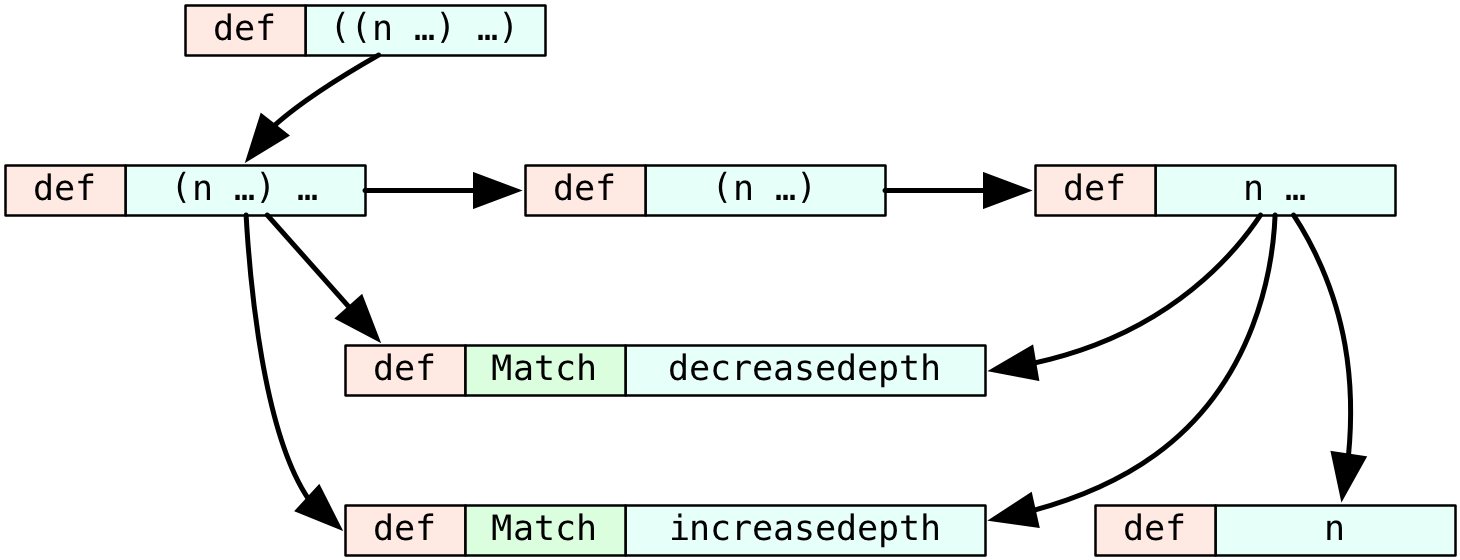
\includegraphics[scale=0.25]{ellipsis-example-callgraph.png}
\caption{Callgraph for function matching pattern \texttt{((n ...) ...)}}
\label{ellipsis-example-callgraph}
\end{figure}

Callgraph for function matching pattern \texttt{((n ...) ...)} can be seen in Figure \ref{ellipsis-example-callgraph}. Code generation algorithm generates five matching functions for this pattern:

\begin{enumerate}
\item function for pattern \texttt{((n ...) ...)}
\item function for pattern \texttt{(n ...) ...}
\item function for pattern \texttt{(n ...) }
\item function for pattern \texttt{n ... }
\item function for pattern \texttt{n}
\end{enumerate}


Figure \ref{ellipsis-example-fig-a} show state of \texttt{Match} object before beggining to match a term (red nodes) against a pattern (blue nodes). Outlined pattern nodes represent current sub-pattern being matched; and since matching hasn't begun yet the entire pattern is outlined.Same applies to the term. Initially, \texttt{Binding} instance assigned to pattern variable \texttt{n} in \texttt{Match} instance has an empty stack.

Figure \ref{ellipsis-example-fig-b} shows state of \texttt{Match} object after entering generated function for \textit{outer} ellipsis and calling \texttt{increasedepth("n")} method. This pushes empty \texttt{TermSequence} onto the stack.


Figure \ref{ellipsis-example-fig-c} shows state of \texttt{Match} object after entering generated function for \textit{inner} ellipsis and calling \texttt{increasedepth("n")} method. This pushes empty \texttt{TermSequence} onto the stack. The term now contains two \texttt{TermSequence} instances.

Figure \ref{ellipsis-example-fig-d} shows matching of term \texttt{Integer(1)}. Need to call \texttt{addtobinding} method with \texttt{"n"} and \texttt{Integer(1)} as arguments. Since topmost term on the stack is \texttt{TermSequence}, \texttt{Integer(1)} is appended to it.

Figures \ref{ellipsis-example-fig-e} and \ref{ellipsis-example-fig-f} call \texttt{addtobinding} with \texttt{Float(2.01)} and \texttt{Integer(3)}. Both terms are appended to the topmost \texttt{TermSequence} on the stack.

All terms in \texttt{TermSequence} have been consumed. Figure \ref{ellipsis-example-fig-g} shows state of the match object after calling \texttt{decreasedepth("n")}. Since the stack contains to \texttt{TermSequence} instances, topmost one is removed from stack and appended to the first \texttt{TermSequence}. Function for \textit{inner} ellipsis is exited.

Now, remaining empty term sequence has to be matched, as seen in Figure \ref{ellipsis-example-fig-h}.

Figure \ref{ellipsis-example-fig-i} shows state of \texttt{Match} object after entering generated function for \textit{inner} ellipsis. Empty \texttt{TermSequence} instance is pushed onto the stack.

However, since term sequence is empty, function for \texttt{Number} pattern cannot be called. Figure \ref{ellipsis-example-fig-j} shows state of the \texttt{Match} object after calling \texttt{decreasedepth("n")}. Since stack contains two \texttt{TermSequence} instances, topmost one is popped from the stack and appended to previous \texttt{TermSequence}. Function for \textit{inner} ellipsis is exited.

Finally, there's no more terms to match in outermost sequence and \texttt{decreasedepth("n")} has to be called, as shown in Figure \ref{ellipsis-example-fig-k}. Since the stack only contains a single term, \texttt{decreasedepth} has no effect.

Assignment \texttt{n = ((1 2 3)())} is matched, as expected.

One may notice that this example doesn't cover non-determinism when matching patterns under ellipsis. When matching term \texttt{(1 2 3)} against pattern \texttt{n ...} (as shown in Figures \ref{ellipsis-example-fig-d}, \ref{ellipsis-example-fig-e}, \ref{ellipsis-example-fig-f}), the matches shown in Figure \ref{ellipsis-example-matches-1} are returned. Recall that when calling a function that matches \texttt{TermSequence}, \texttt{head} and \texttt{tail} are set to zero and the length of \texttt{TermSequence}, in this case three. Function for \texttt{n ...} is then called, \texttt{increasedepth} method is called on \texttt{match} instance and it is placed into the queue. Match is then popped from the queue, add function for pattern \texttt{n} is called with complete copy of the match. Such repeated copying and calling \texttt{decreasedepth} for each resulting match produces matches shown in Figure \ref{ellipsis-example-matches-1}. Now, when exiting function for pattern \texttt{(n ...)}, only accept matches where \texttt{head=tail}, and there's only such match.

When control flow returns to function for pattern \texttt{(n ...) ...)}, the only returned match is added to the queue. Queue at this point contains a single match. This match is dequeued, and function for pattern \texttt{(n ...) is called} with term \texttt{()}. \texttt{head} and \text{tail} are set to zero and function for pattern \texttt{n ...} is called. \texttt{increasedepth} is called. Since term \texttt{()} contains no numbers, the only possible match returned by this function is shown in Figure \ref{ellipsis-example-matches-2}.

Finally, \textit{outer} ellipsis produces matches shown in Figure \ref{ellipsis-example-matches-3} When returning from function for pattern \texttt{((n ...) ...)}, two of the matches are discarded because \texttt{head != tail}.


\begin{figure}[H]
\caption{Lifetime of match object}
%\begin{adjustwidth}{-1cm}{1cm}
\fbox{
	\begin{subfigure}{0.5\linewidth}
		\raisebox{5mm}{
			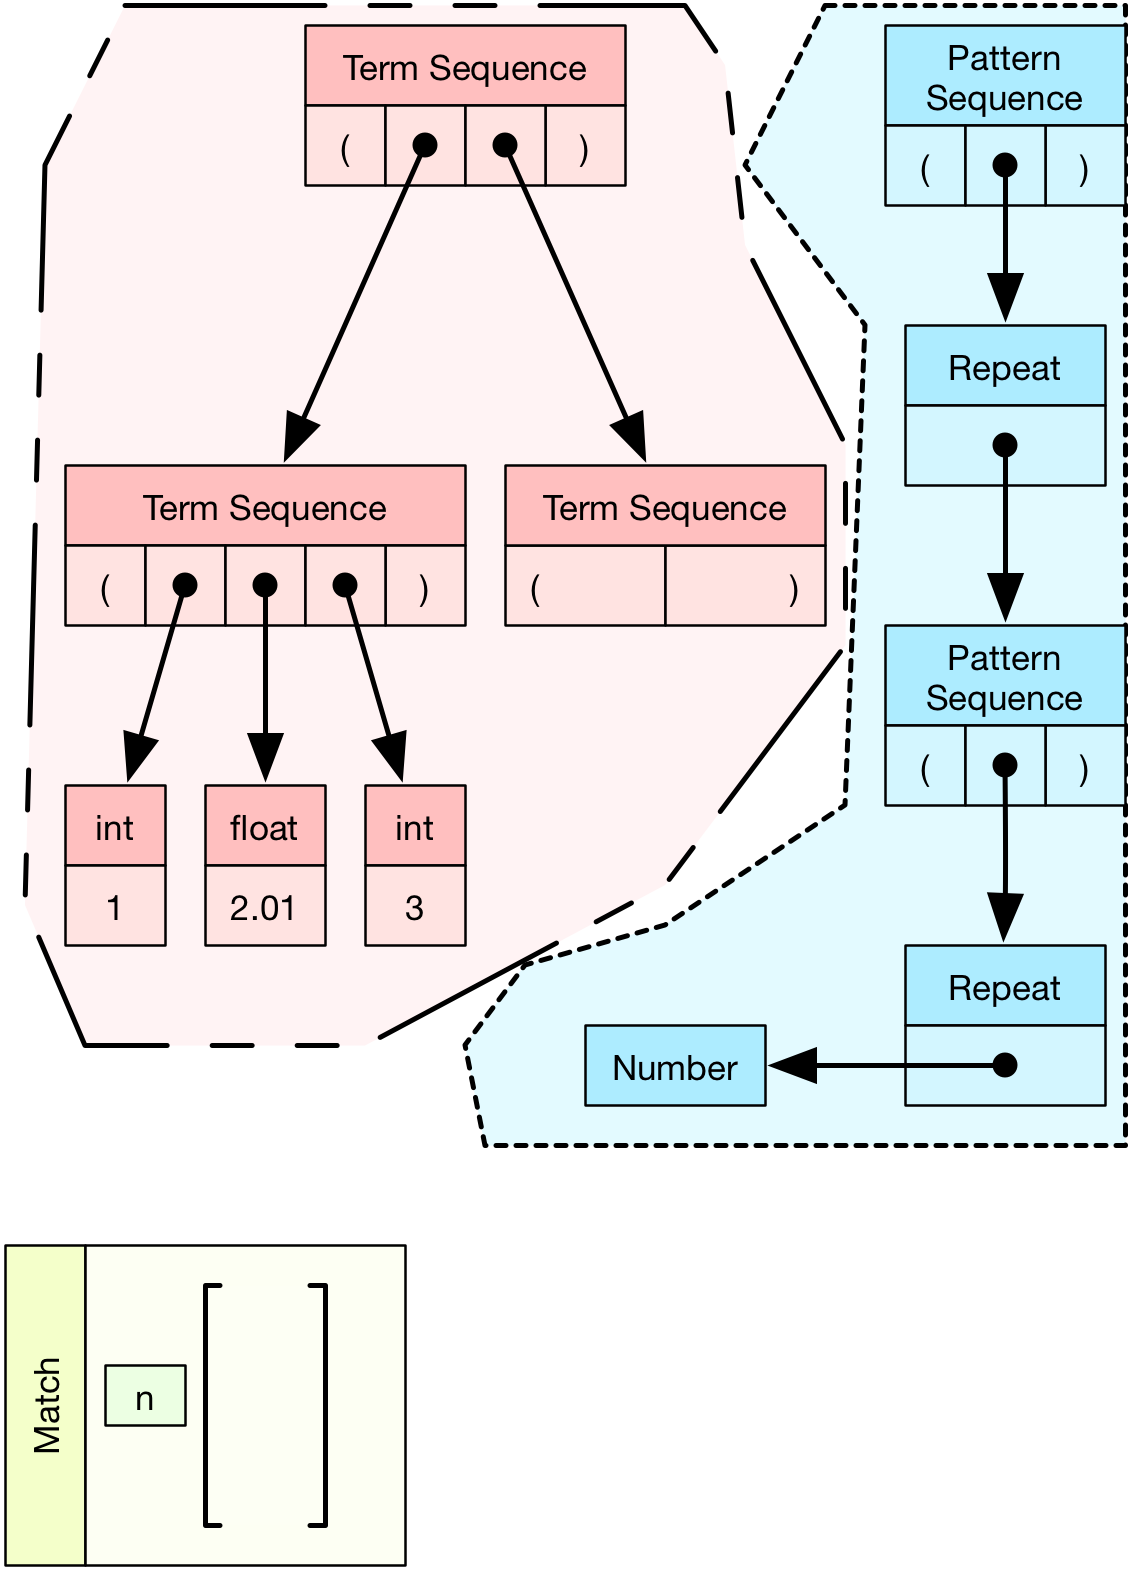
\includegraphics[scale=0.152]{ellipsis-example-fig-a.png}
		}
		\caption{Before matching the pattern.}
		\label{ellipsis-example-fig-a}
	\end{subfigure}
	\begin{subfigure}{0.5\linewidth}
		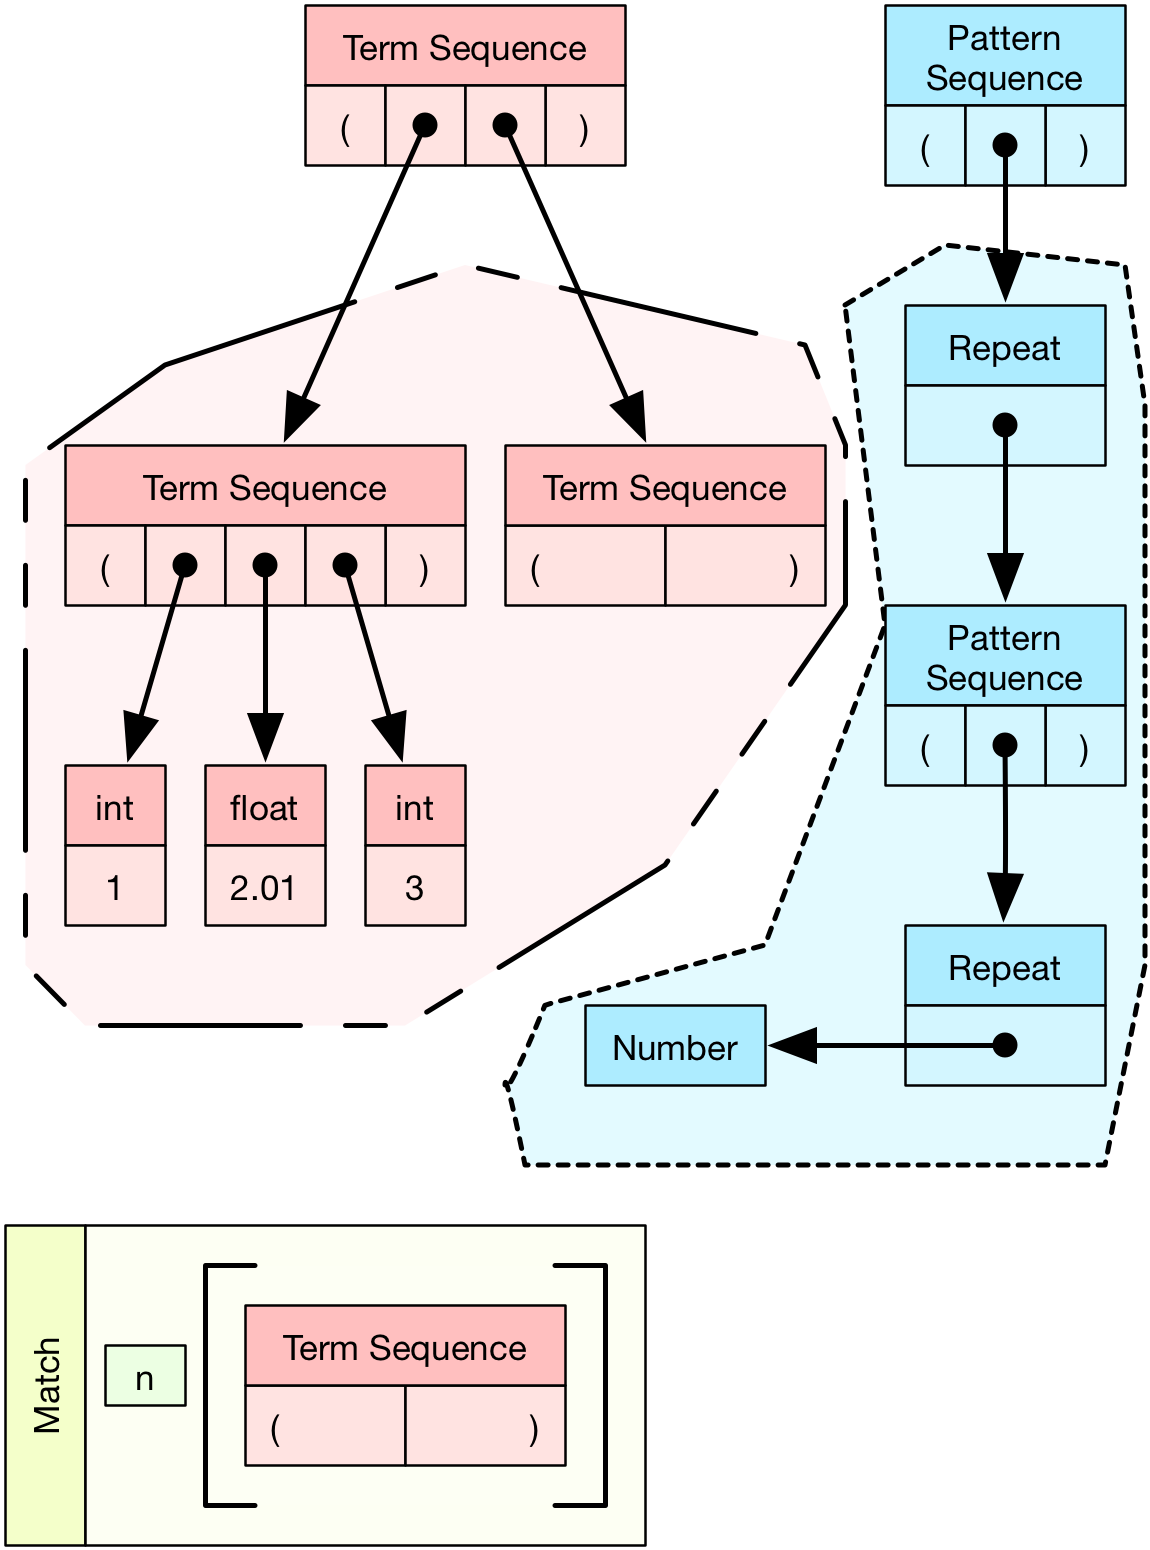
\includegraphics[scale=0.152]{ellipsis-example-fig-b.png}
		\caption{Enter outer ellipsis and \texttt{increasedepth("n")}.}
		\label{ellipsis-example-fig-b}
	\end{subfigure}
}

\fbox{
	\begin{subfigure}{0.5\linewidth}
		\raisebox{19mm}{
			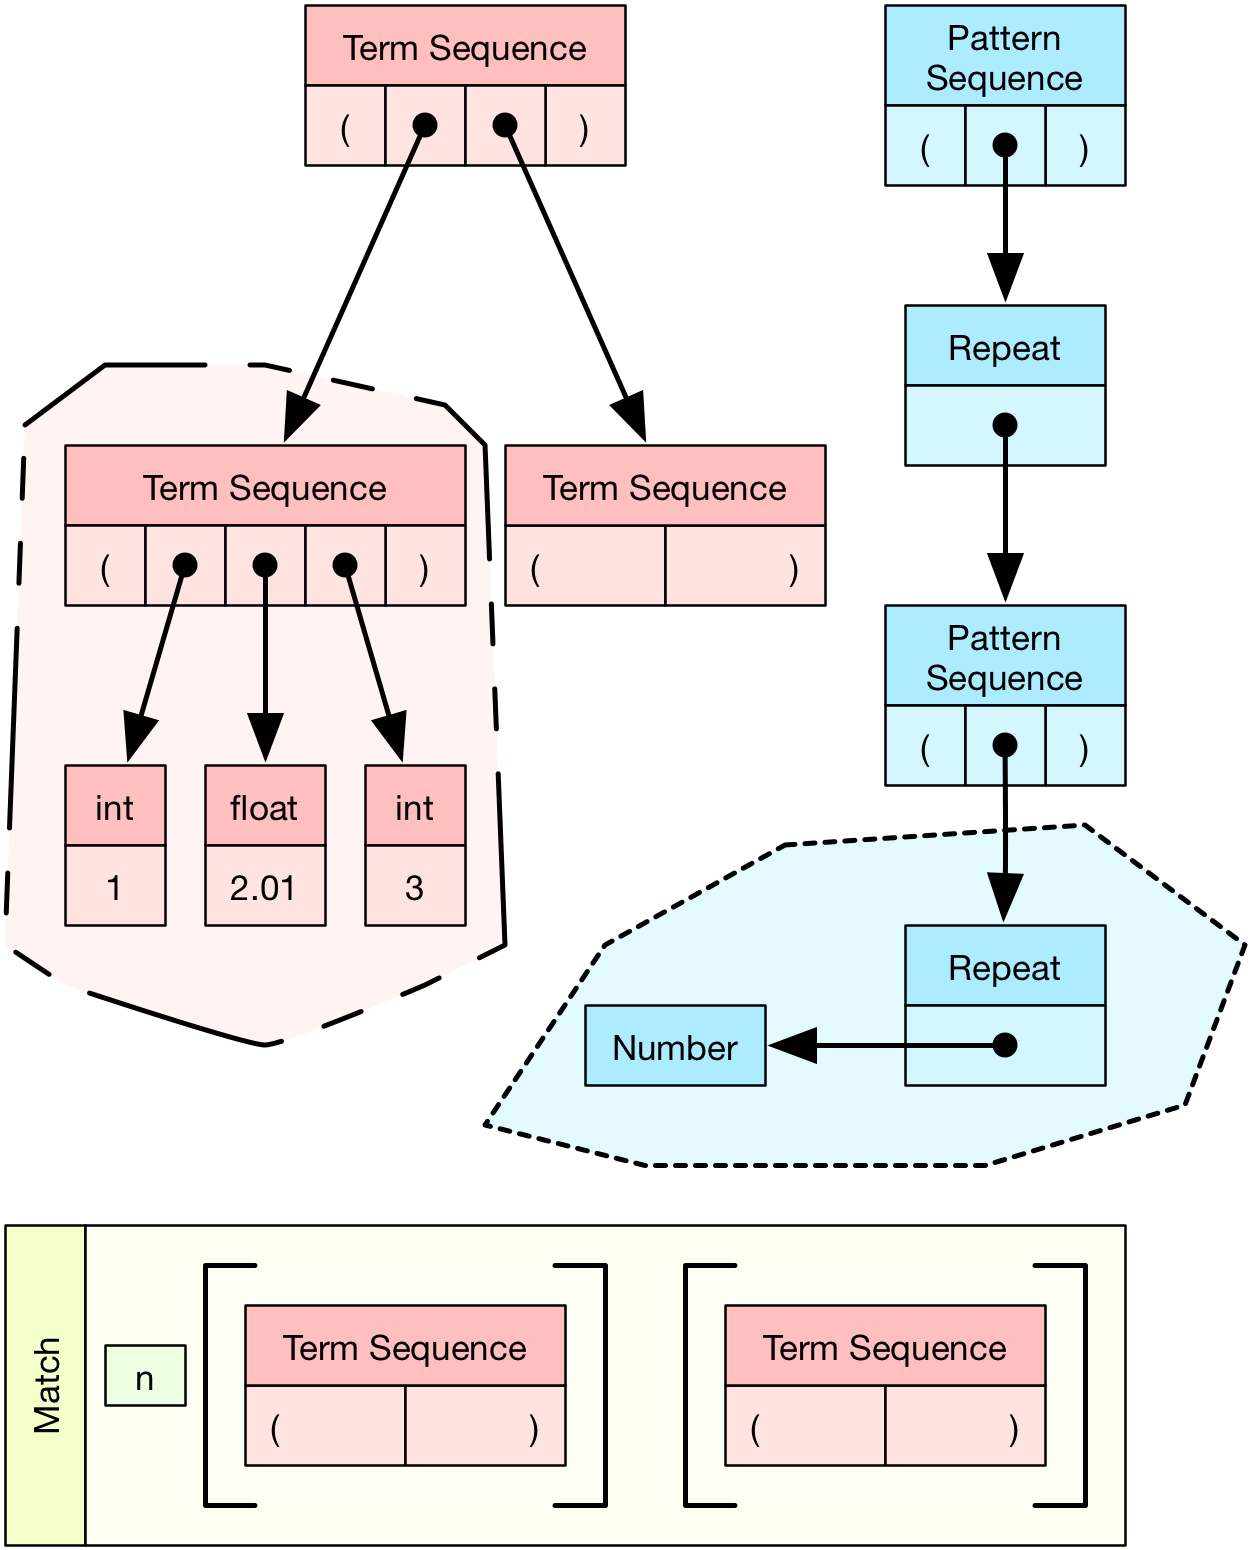
\includegraphics[scale=0.152]{ellipsis-example-fig-c.png}
		}
		\caption{Enter inner ellipsis and \texttt{increasedepth("n")}.}
		\label{ellipsis-example-fig-c}
	\end{subfigure}
	\begin{subfigure}{0.5\linewidth}
		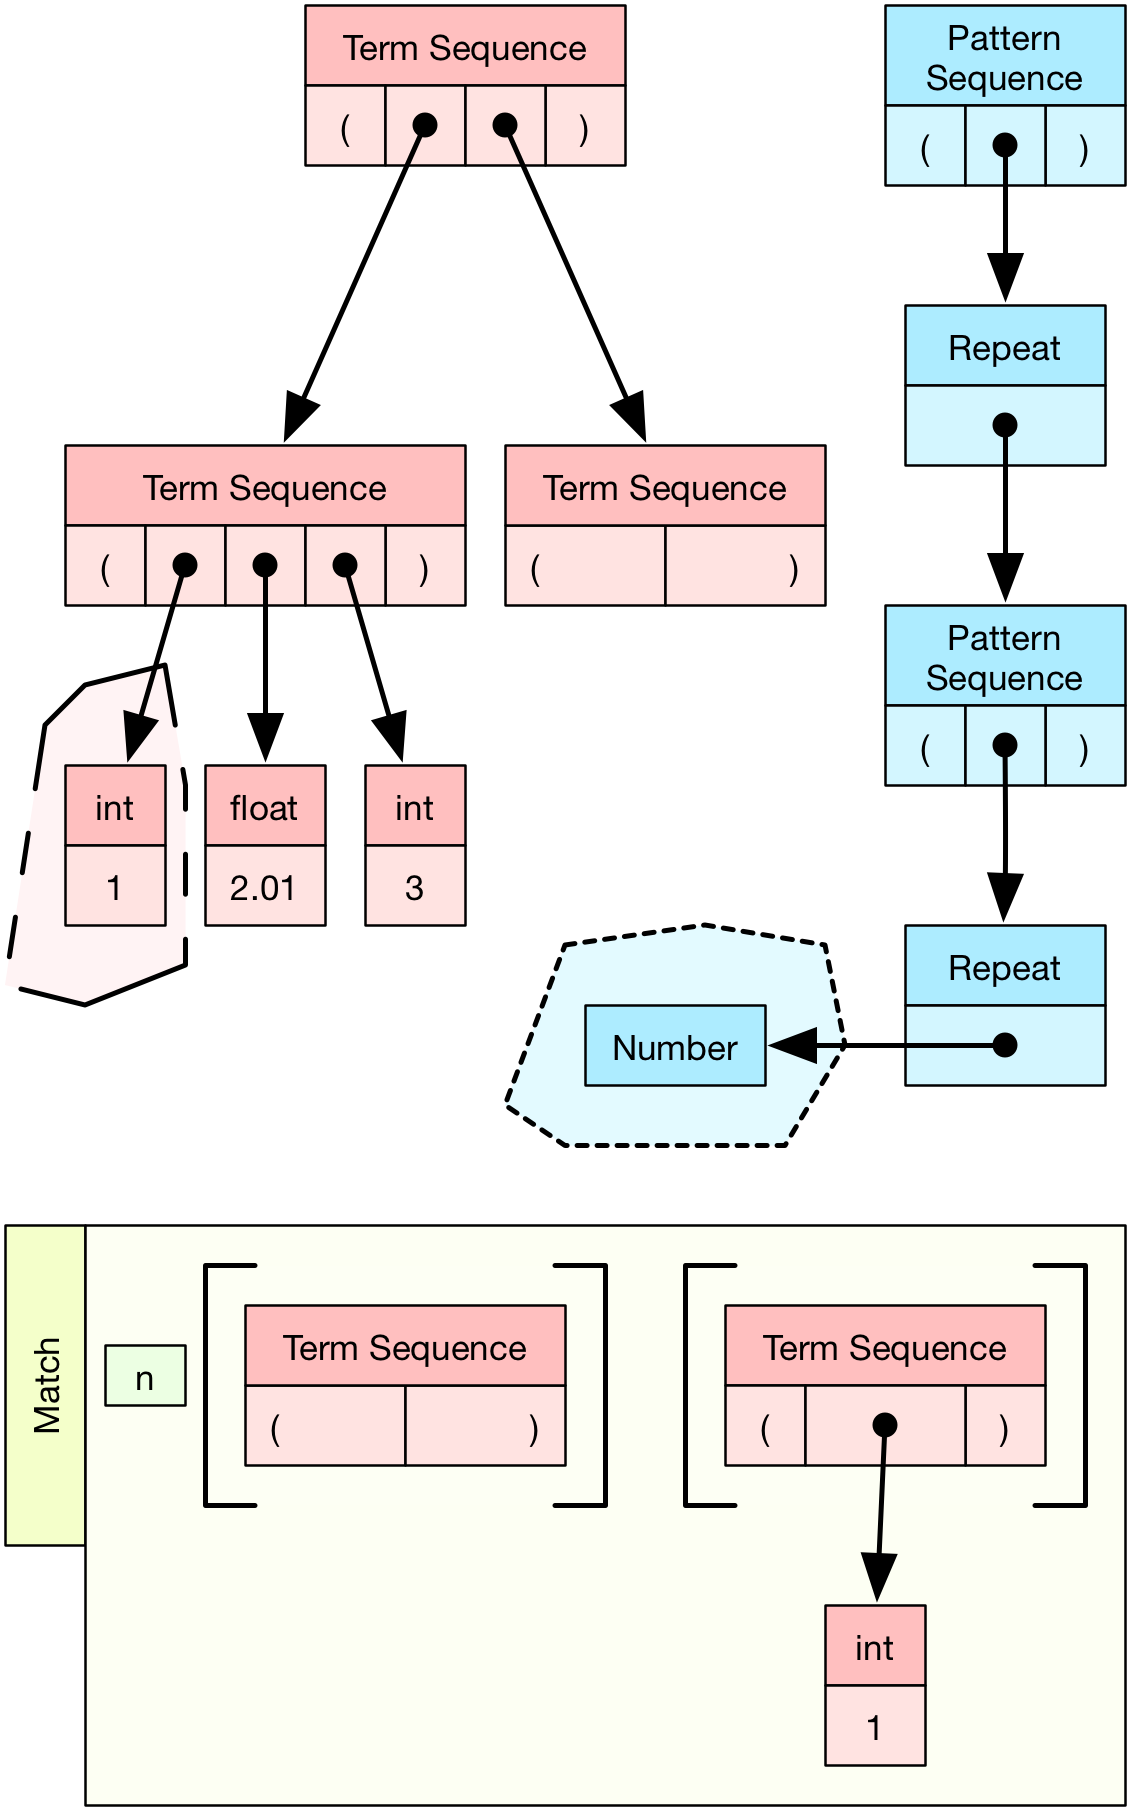
\includegraphics[scale=0.152]{ellipsis-example-fig-d.png}
		\caption{\texttt{addtobinding("n", Integer(1))}}
		\label{ellipsis-example-fig-d}
	\end{subfigure}
}

%\end{adjustwidth}
\end{figure}

\begin{figure}[H]\ContinuedFloat
\fbox{
	\begin{subfigure}{0.5\linewidth}
		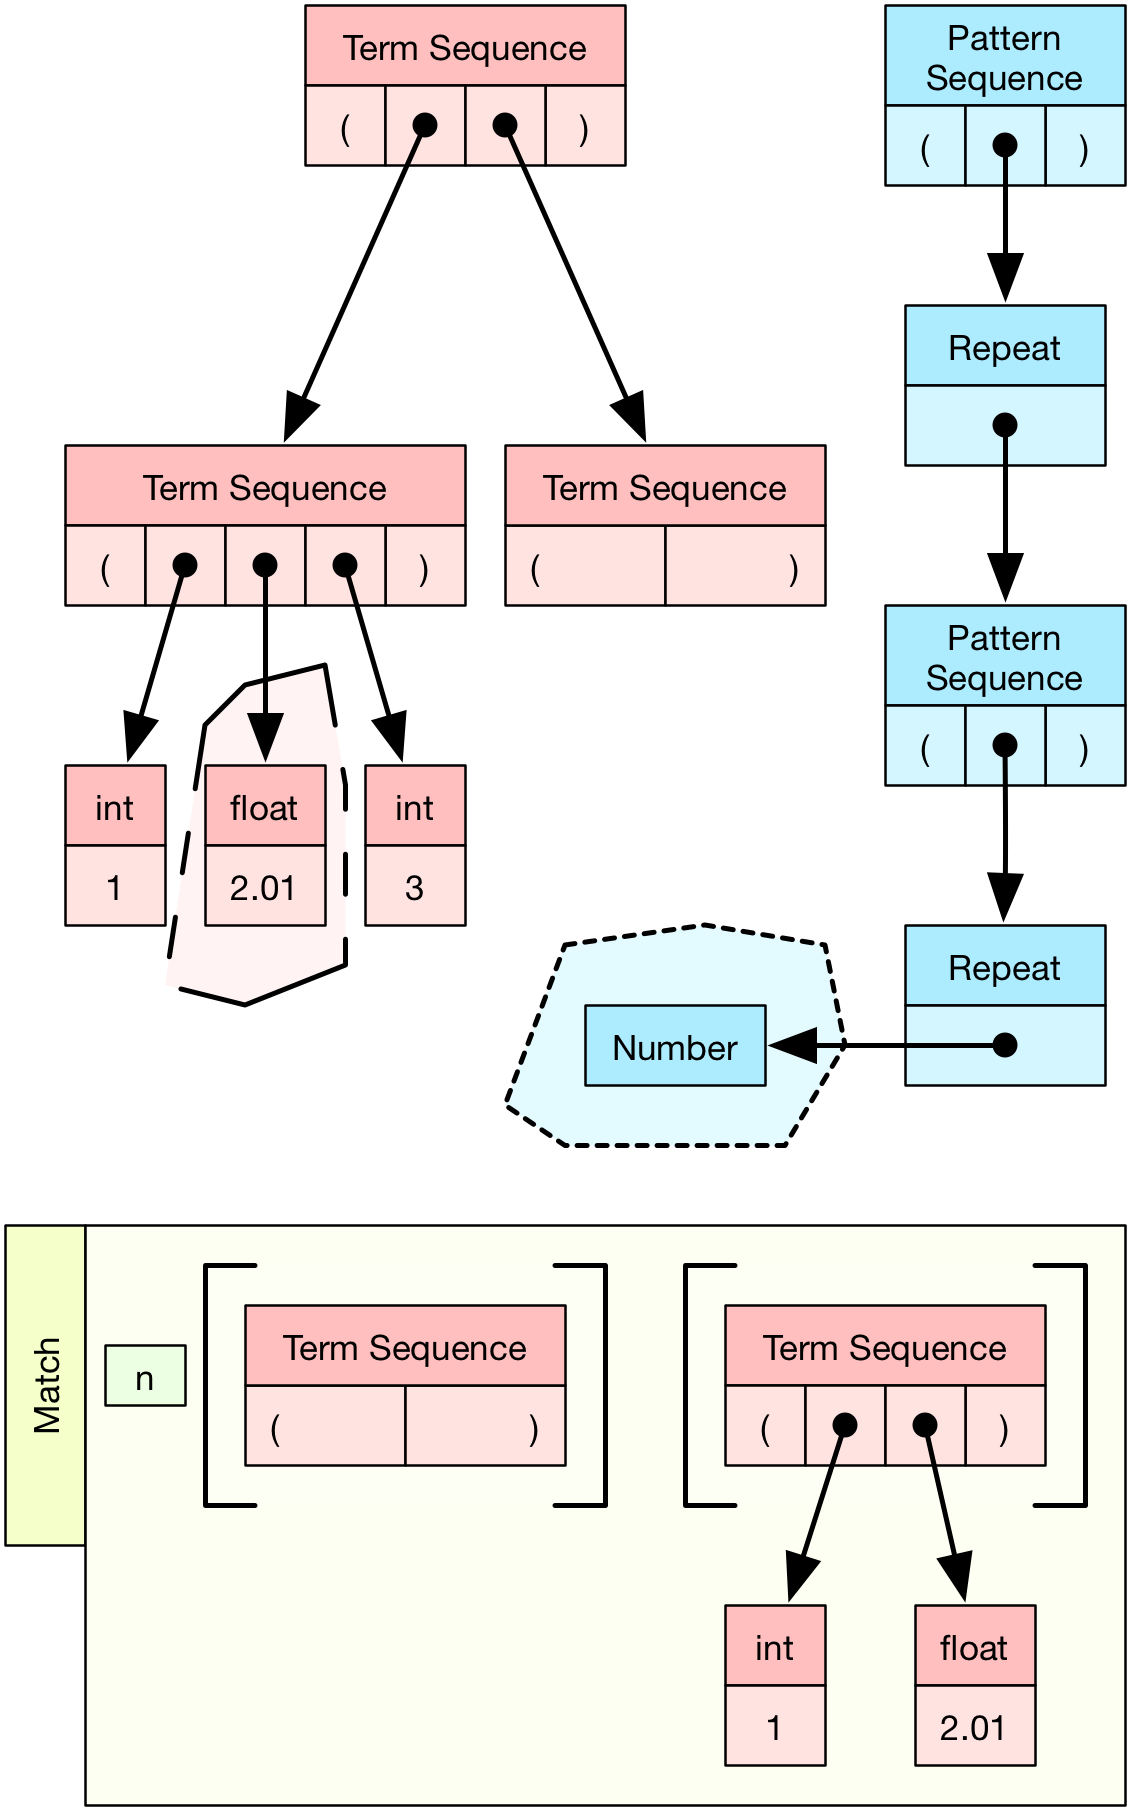
\includegraphics[scale=0.152]{ellipsis-example-fig-e.png}
		\caption{\texttt{addtobinding("n", Float(2.01))}}
		\label{ellipsis-example-fig-e}
	\end{subfigure}
	\begin{subfigure}{0.5\linewidth}
		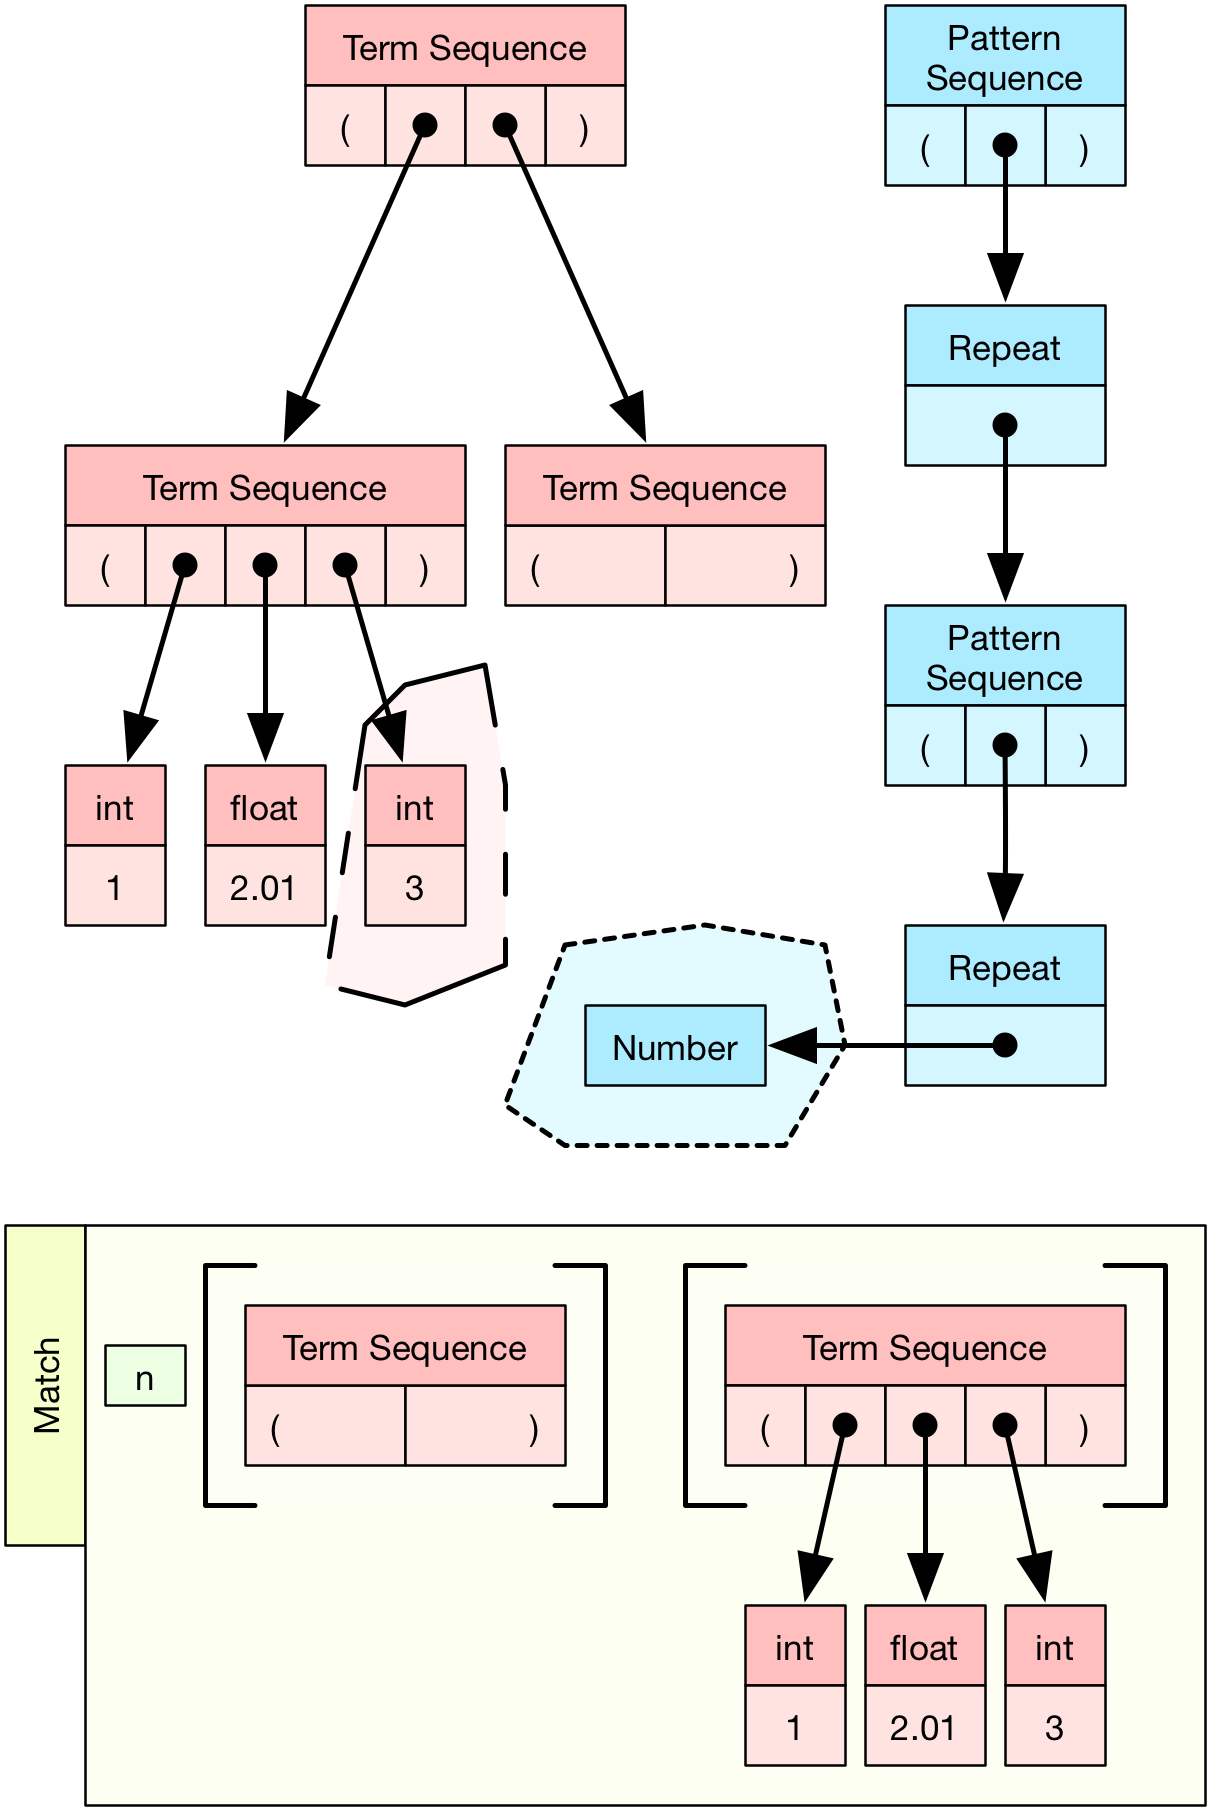
\includegraphics[scale=0.152]{ellipsis-example-fig-f.png}
		\caption{\texttt{addtobinding("n", Integer(3))}}
		\label{ellipsis-example-fig-f}
	\end{subfigure}
}
\fbox{
\begin{subfigure}{0.5\linewidth}
	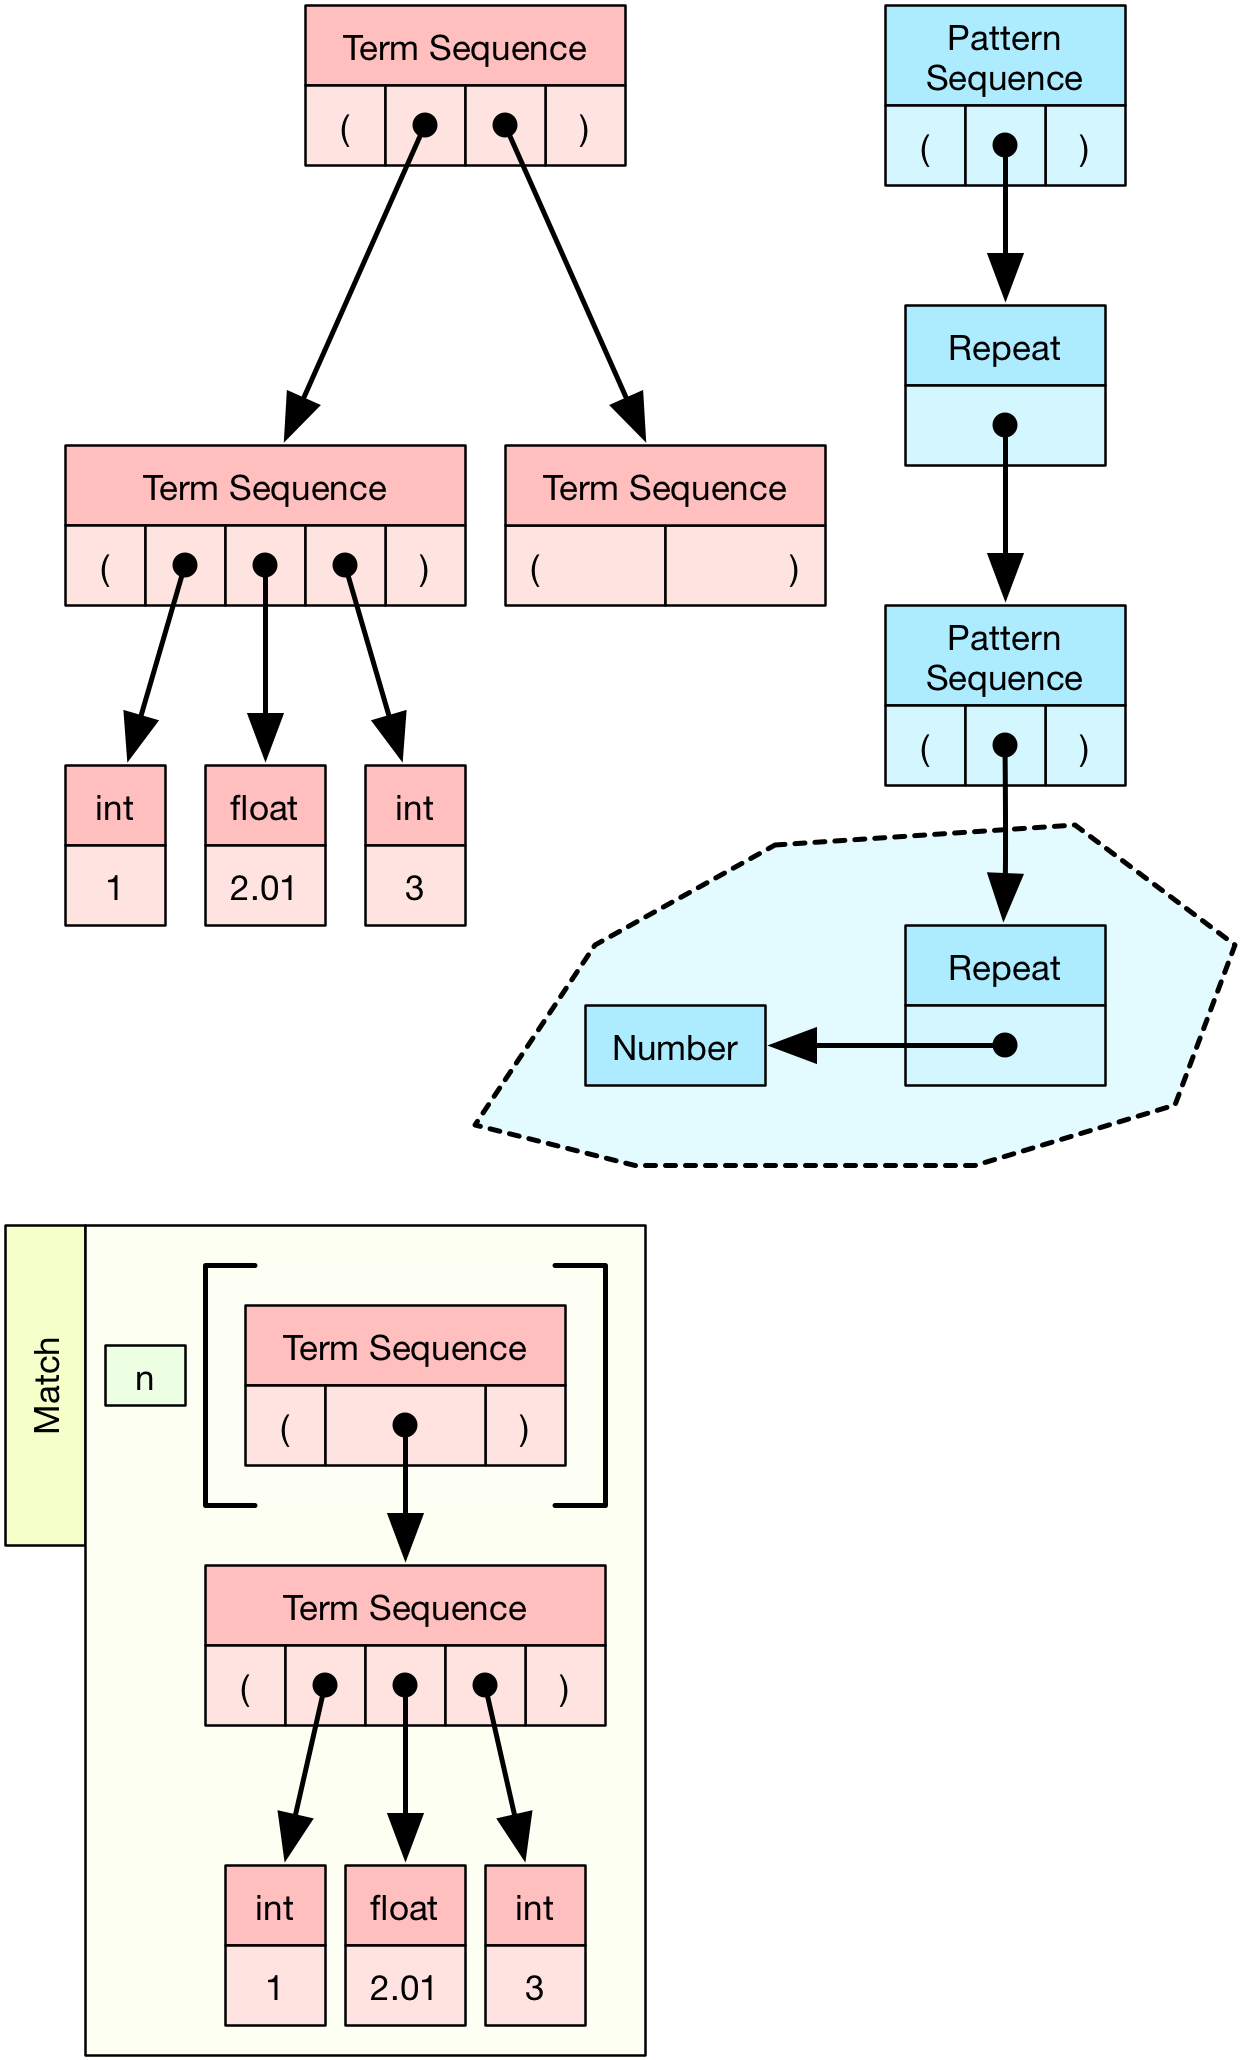
\includegraphics[scale=0.152]{ellipsis-example-fig-g.png}
	\caption{\texttt{decreasedepth("n")} and leave inner ellipsis.}
	\label{ellipsis-example-fig-g}
\end{subfigure}
\begin{subfigure}{0.5\linewidth}
	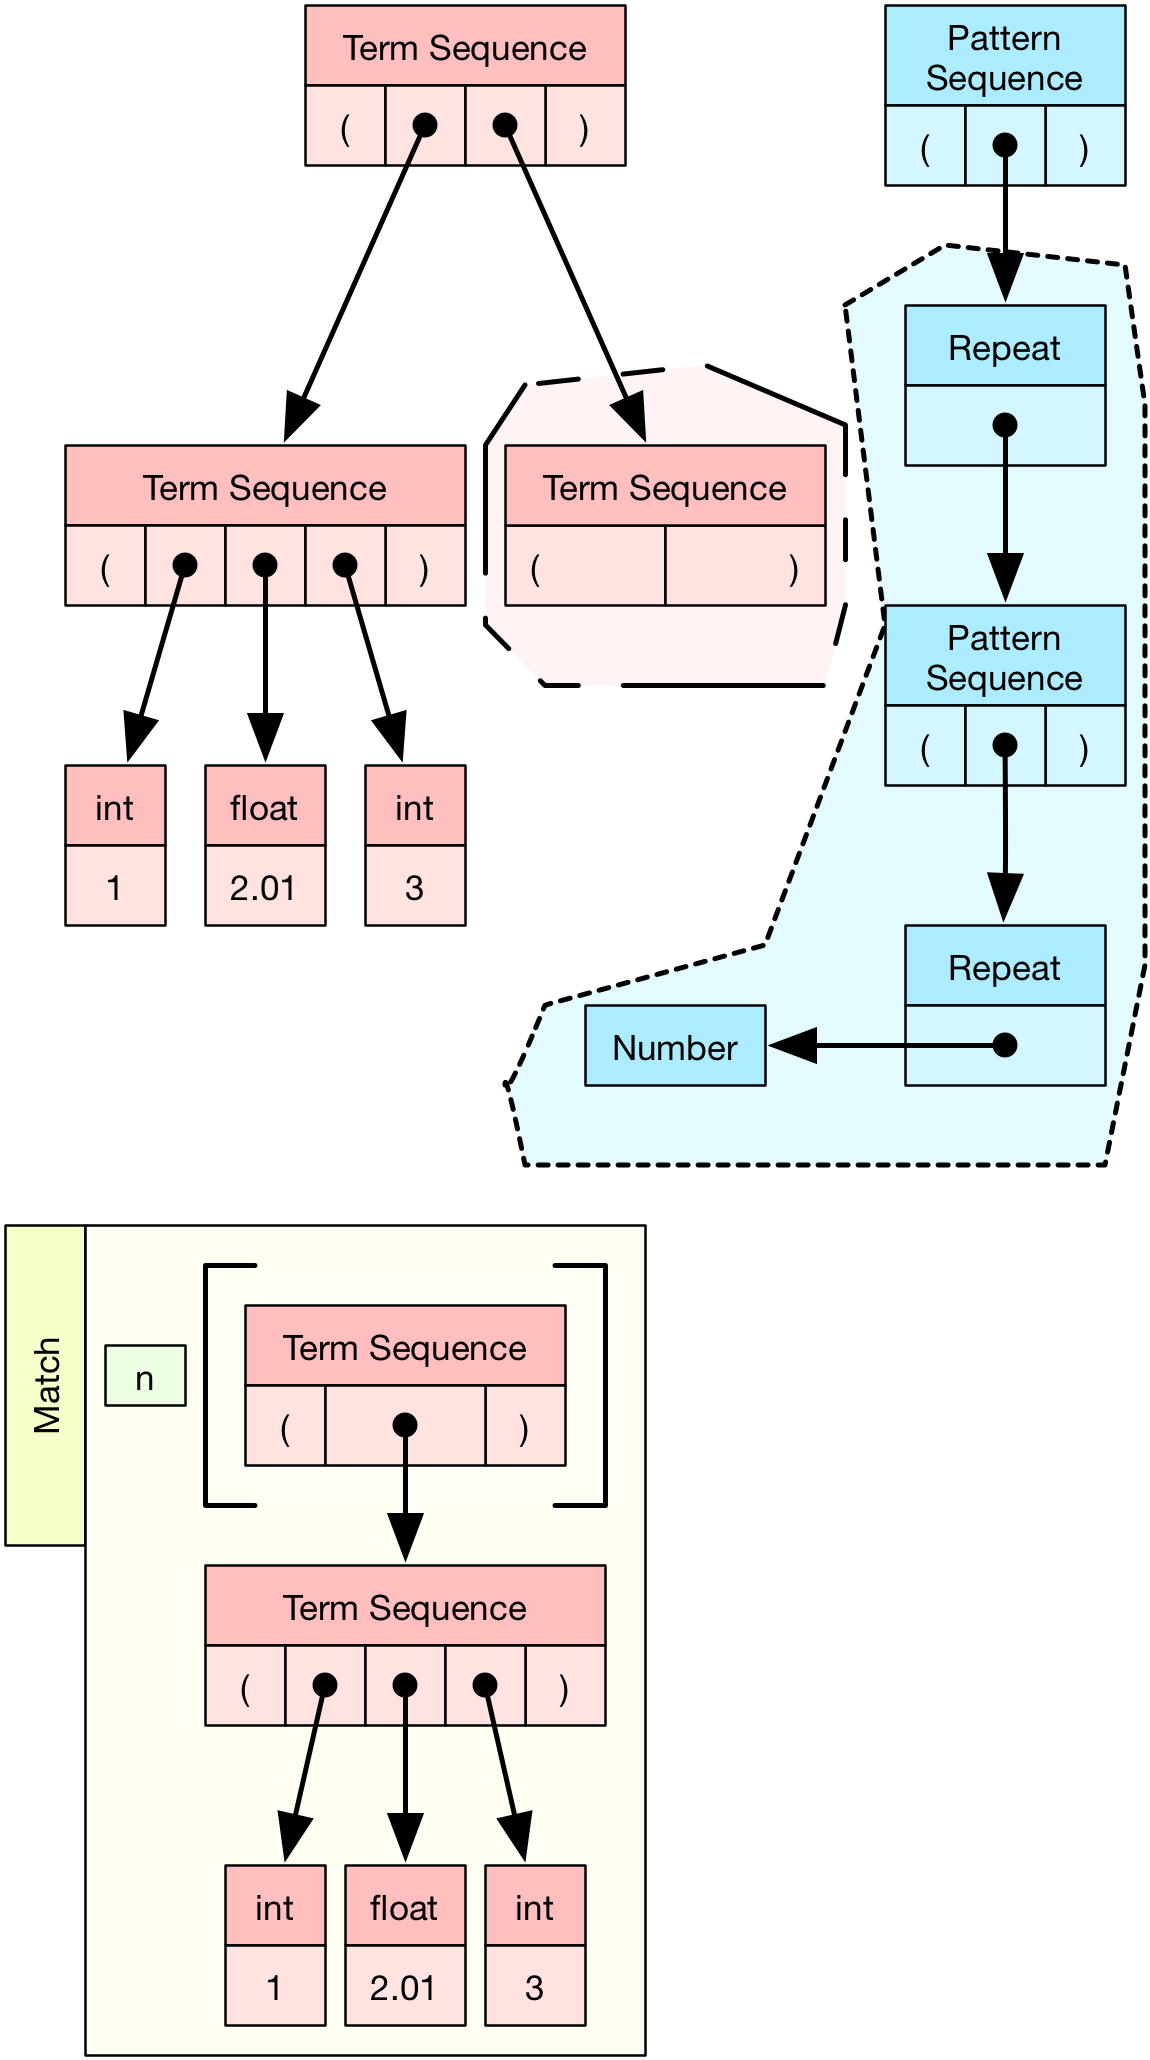
\includegraphics[scale=0.152]{ellipsis-example-fig-h.png}
	\caption{Start processing the next term in the sequence.}
	\label{ellipsis-example-fig-h}
\end{subfigure}
}
\end{figure}
\begin{figure}[H]\ContinuedFloat
\fbox{
	\begin{subfigure}{0.5\linewidth}
		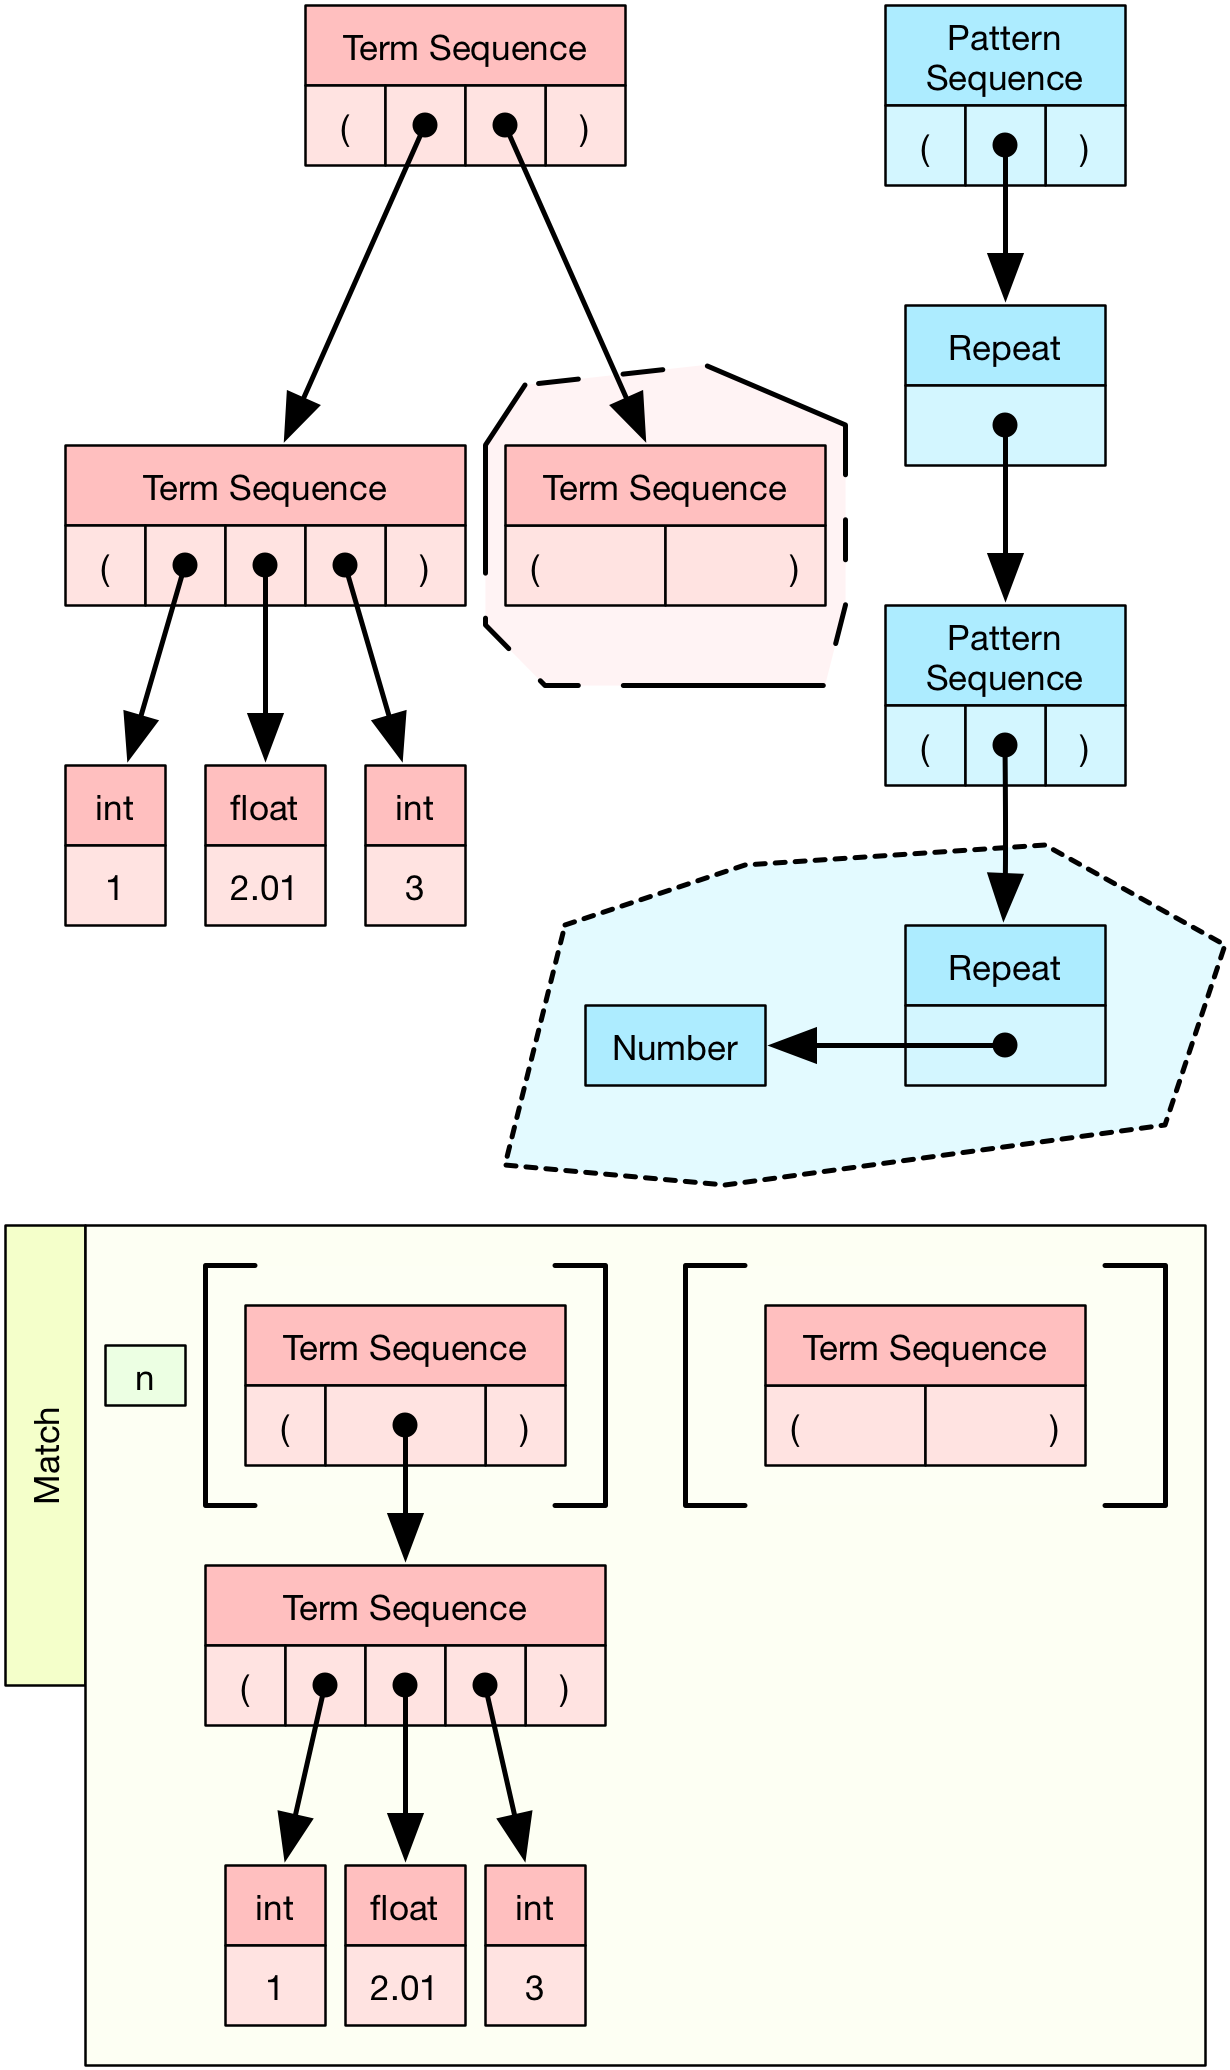
\includegraphics[scale=0.152]{ellipsis-example-fig-i.png}
		\caption{\texttt{increasedepth("n")} after entering inner ellipsis.}
		\label{ellipsis-example-fig-i}
	\end{subfigure}
	\begin{subfigure}{0.5\linewidth}
		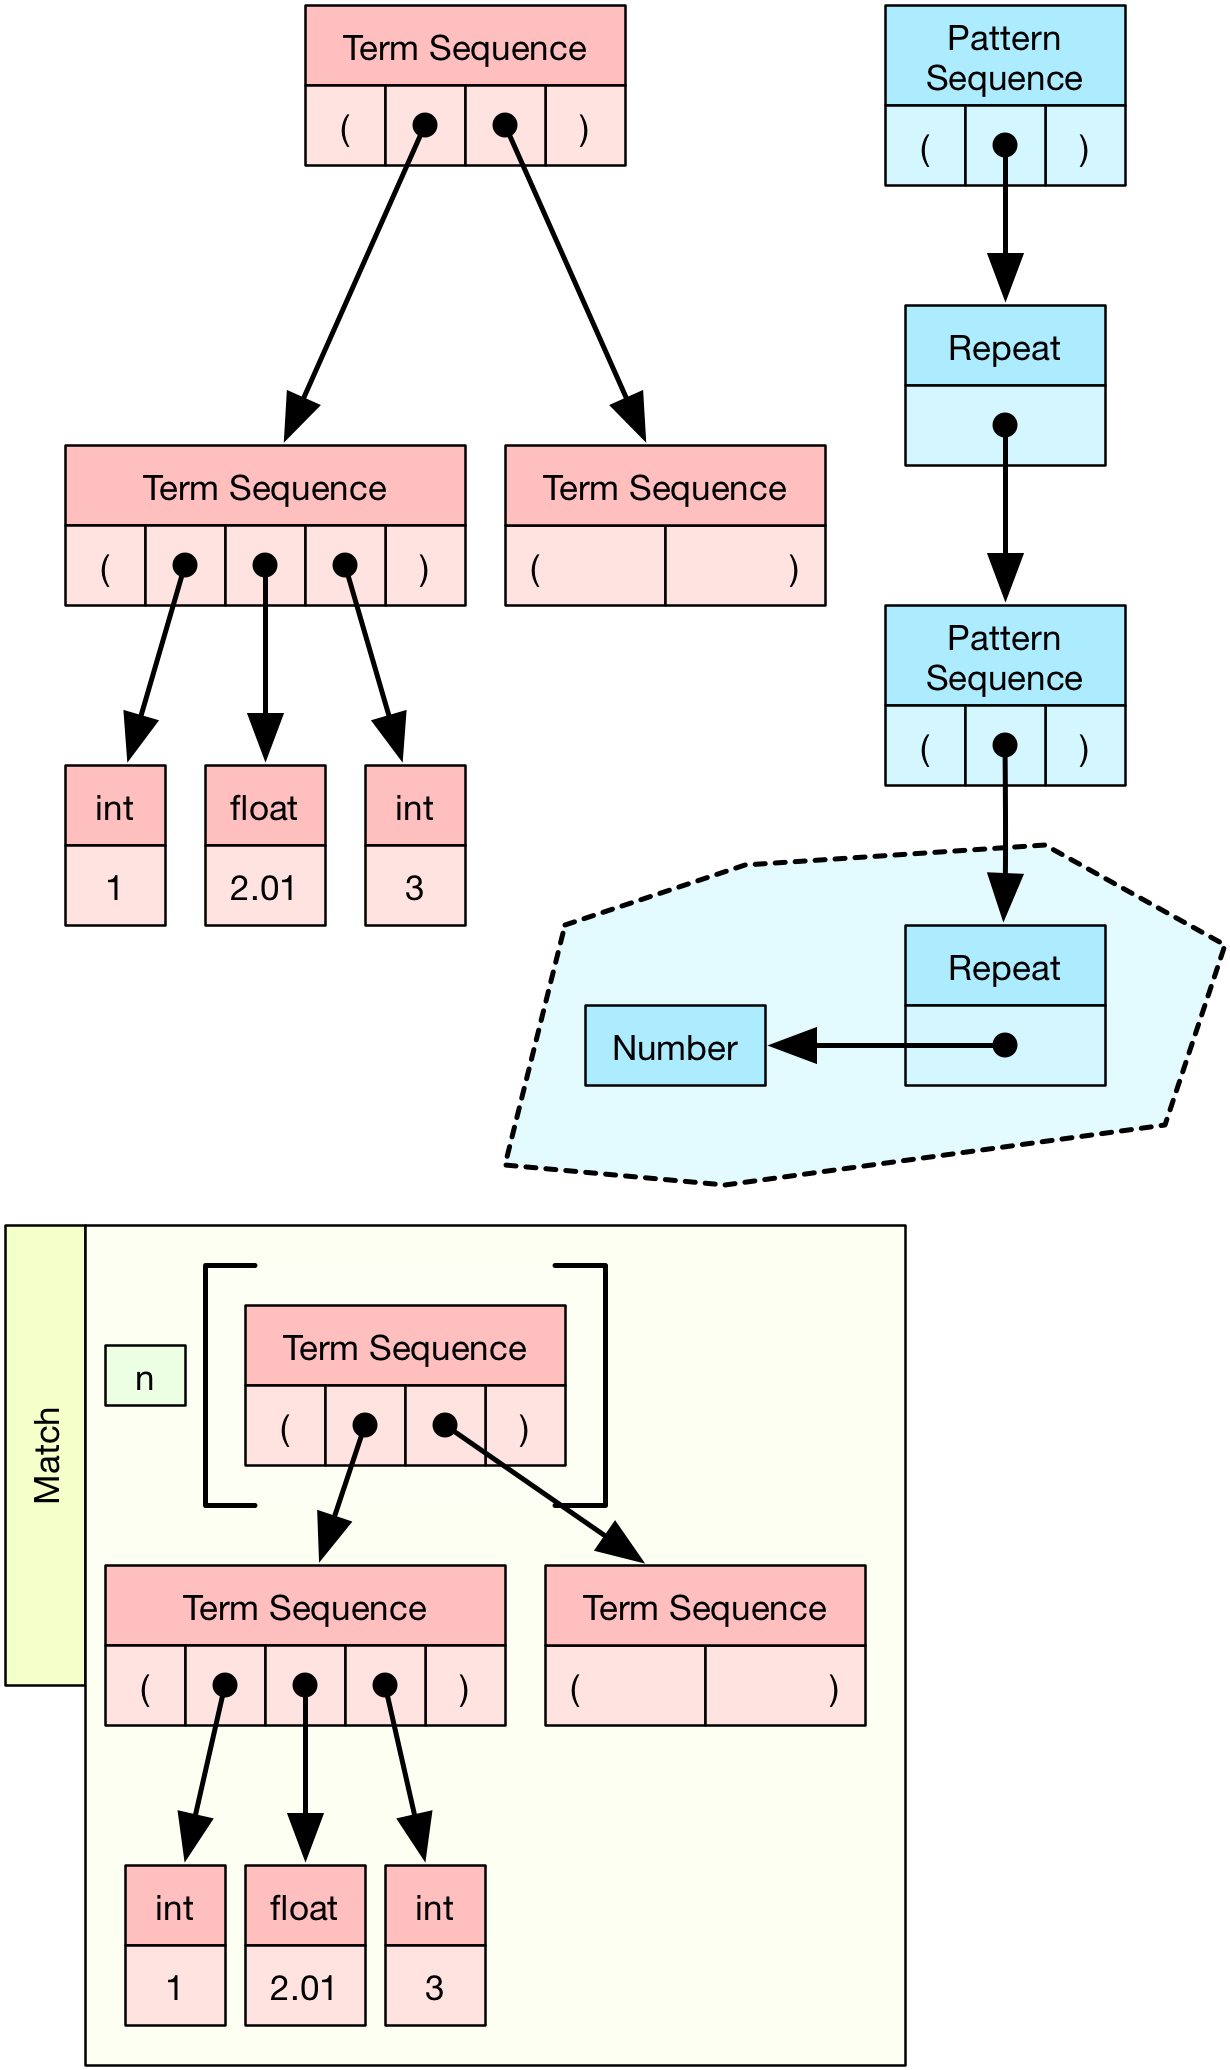
\includegraphics[scale=0.152]{ellipsis-example-fig-j.png}
		\caption{\texttt{decreasedepth("n")} and leave inner ellipsis.}
		\label{ellipsis-example-fig-j}
	\end{subfigure}
}

\fbox{
	\begin{subfigure}{0.5\linewidth}
		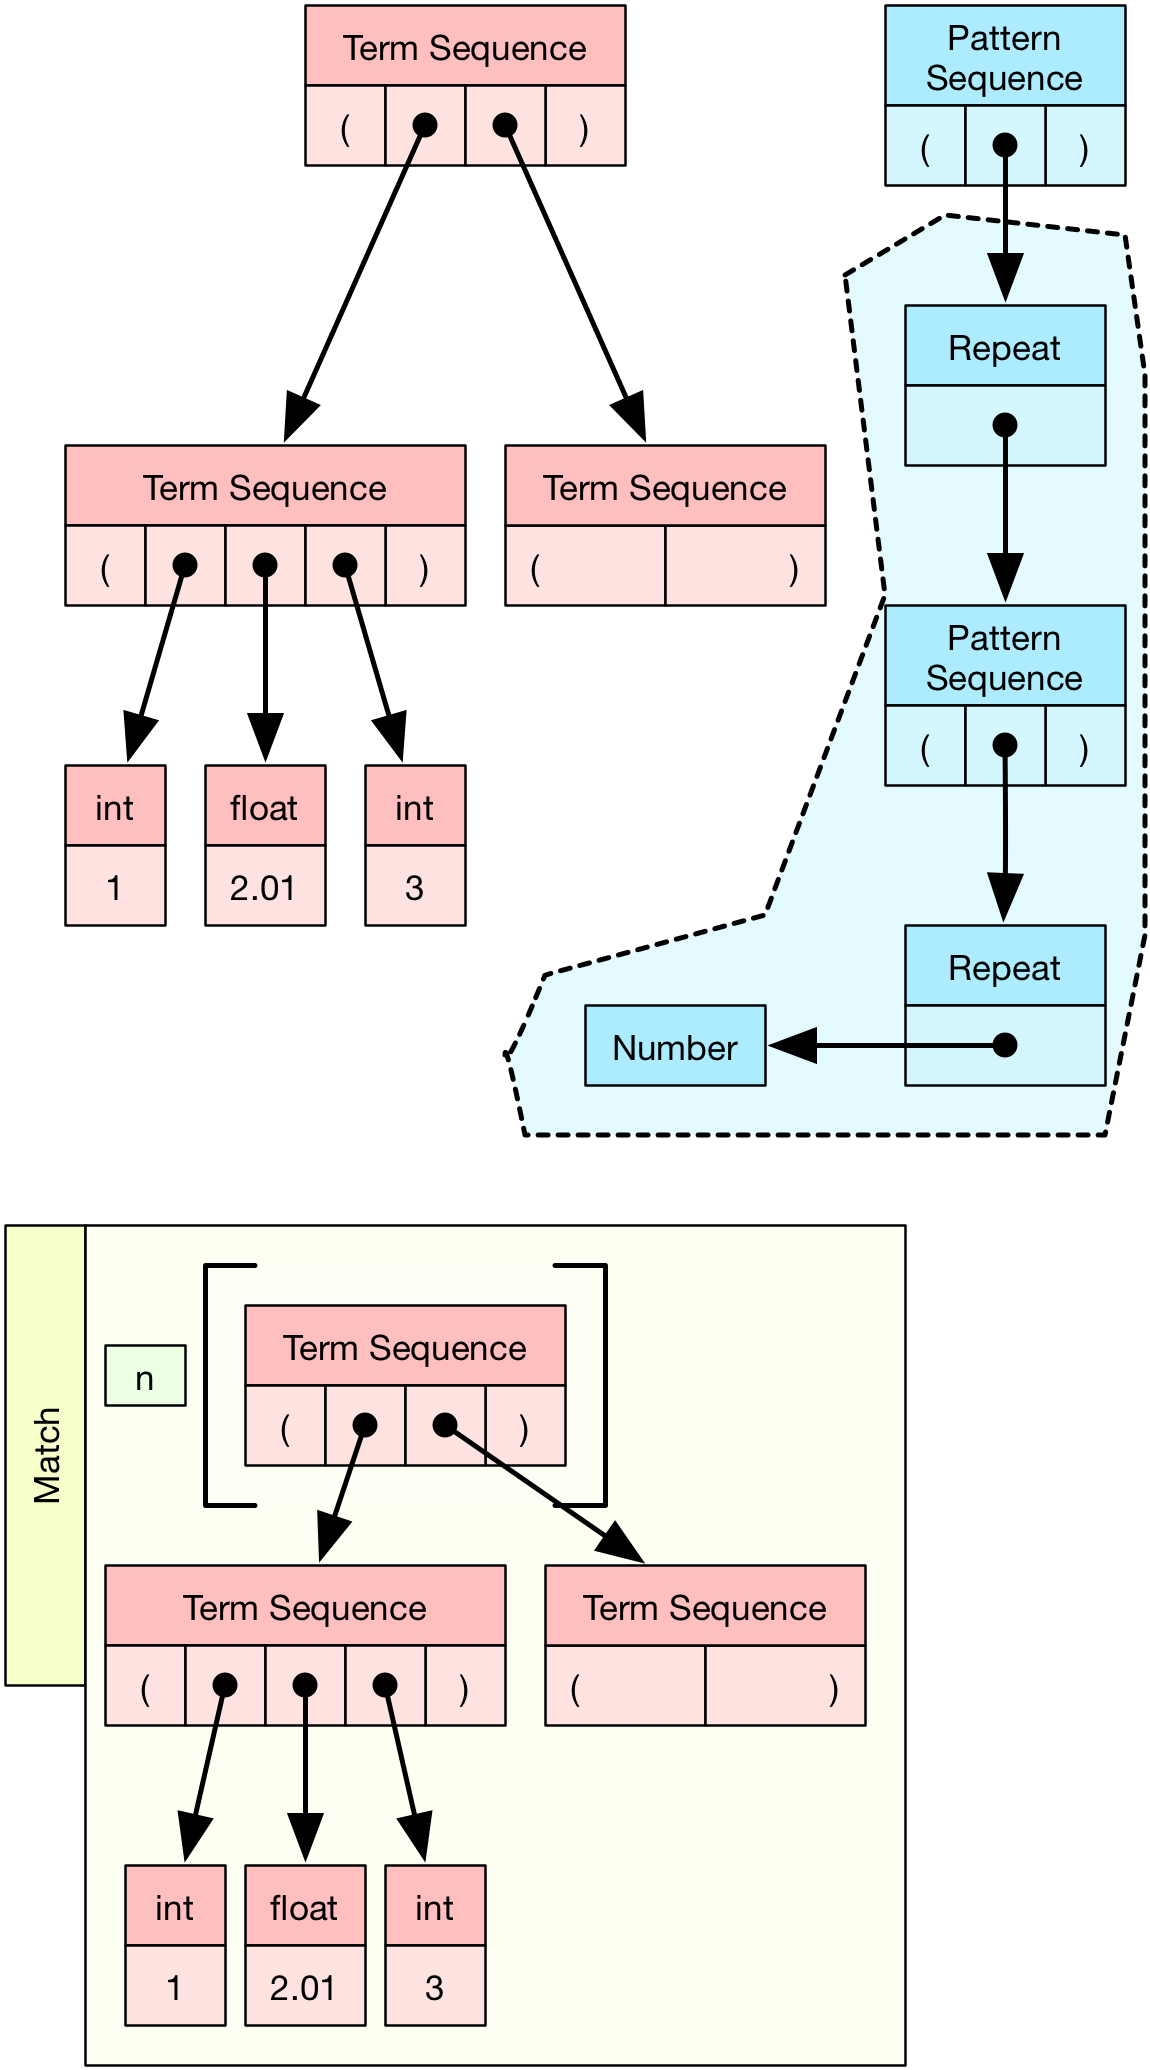
\includegraphics[scale=0.152]{ellipsis-example-fig-k.png}
		\caption{\texttt{decreasedepth("n") and leave outer ellipsis}.}
		\label{ellipsis-example-fig-k}
	\end{subfigure}
}

\end{figure}

\begin{figure}[h]
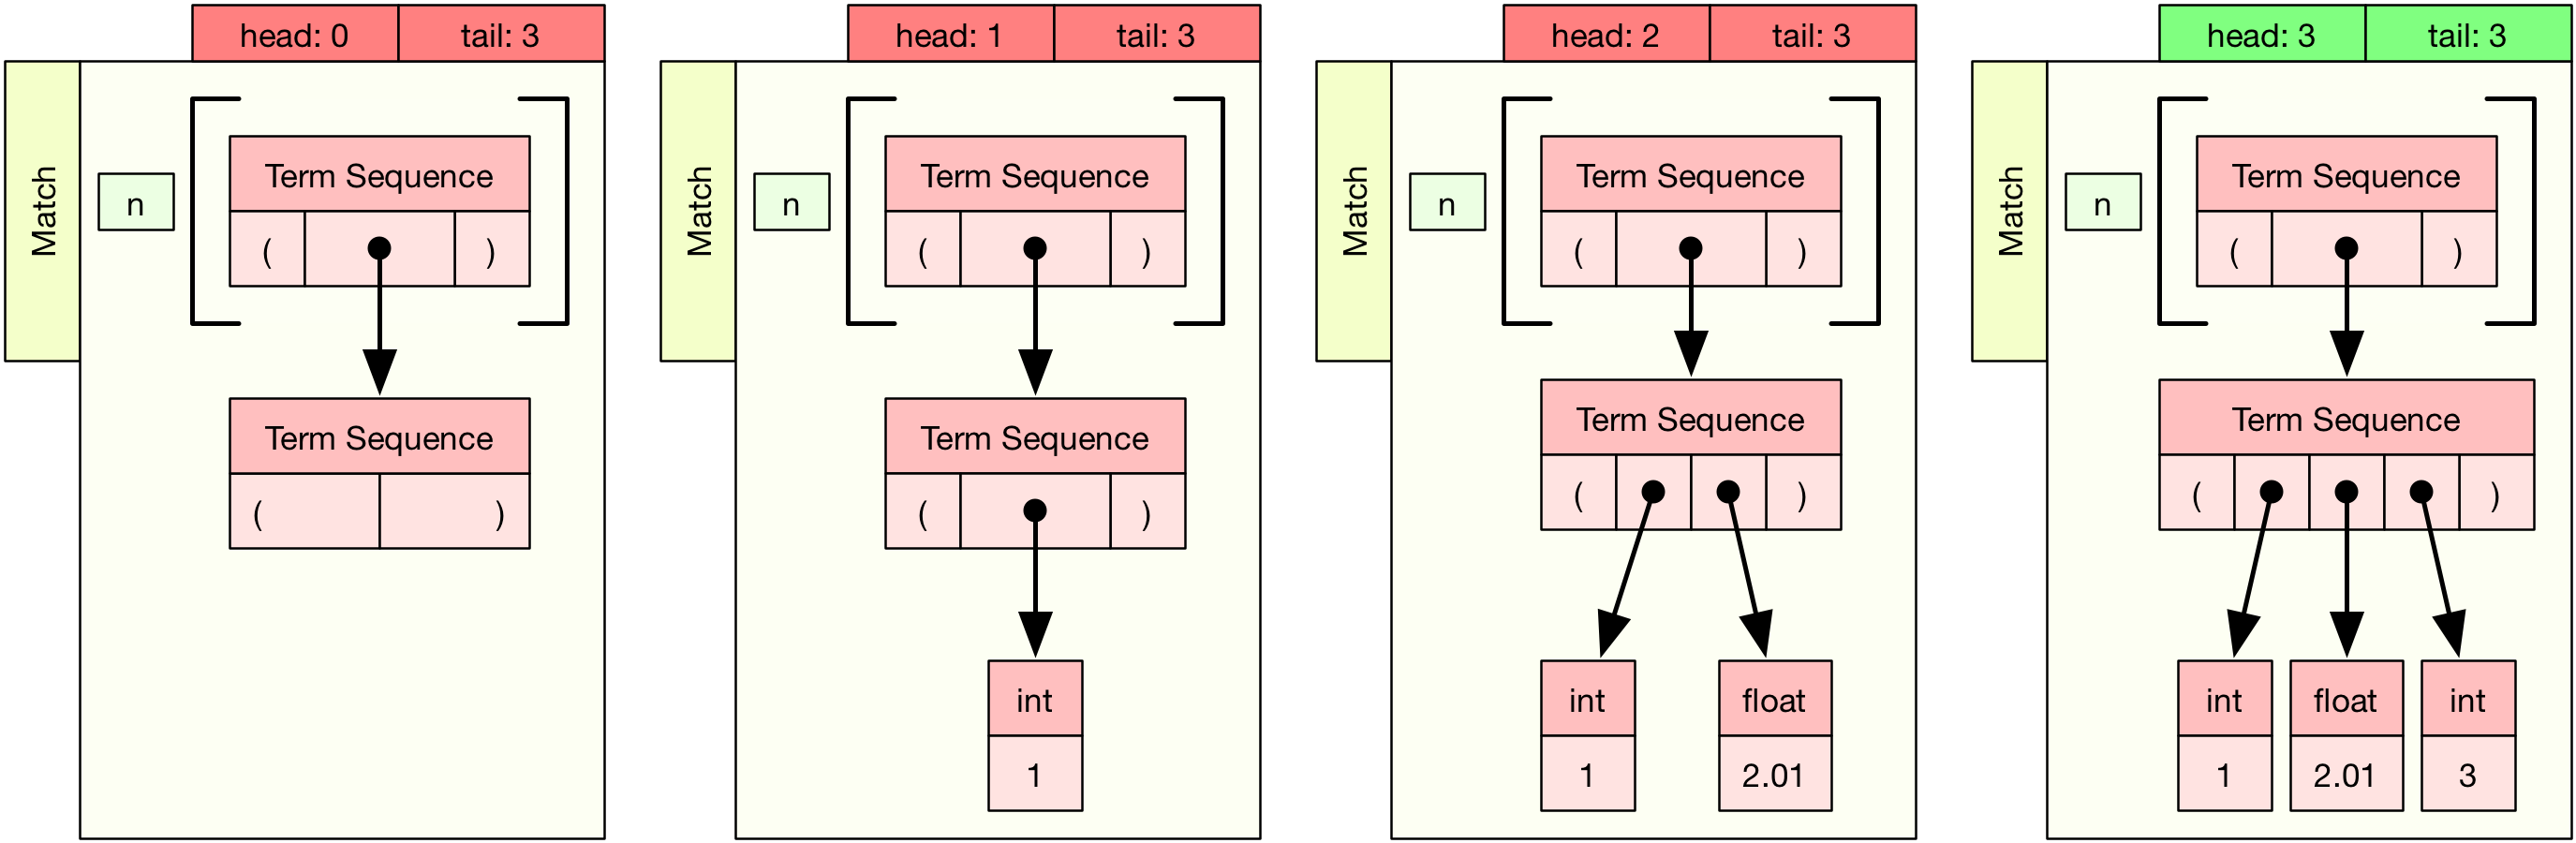
\includegraphics[scale=0.152]{ellipsis-example-matches-1.png}
\caption{Matches returned after matching term \texttt{(1 2 3)} against pattern \texttt{n ...}}
\label{ellipsis-example-matches-1}
\end{figure}


\begin{figure}[h]
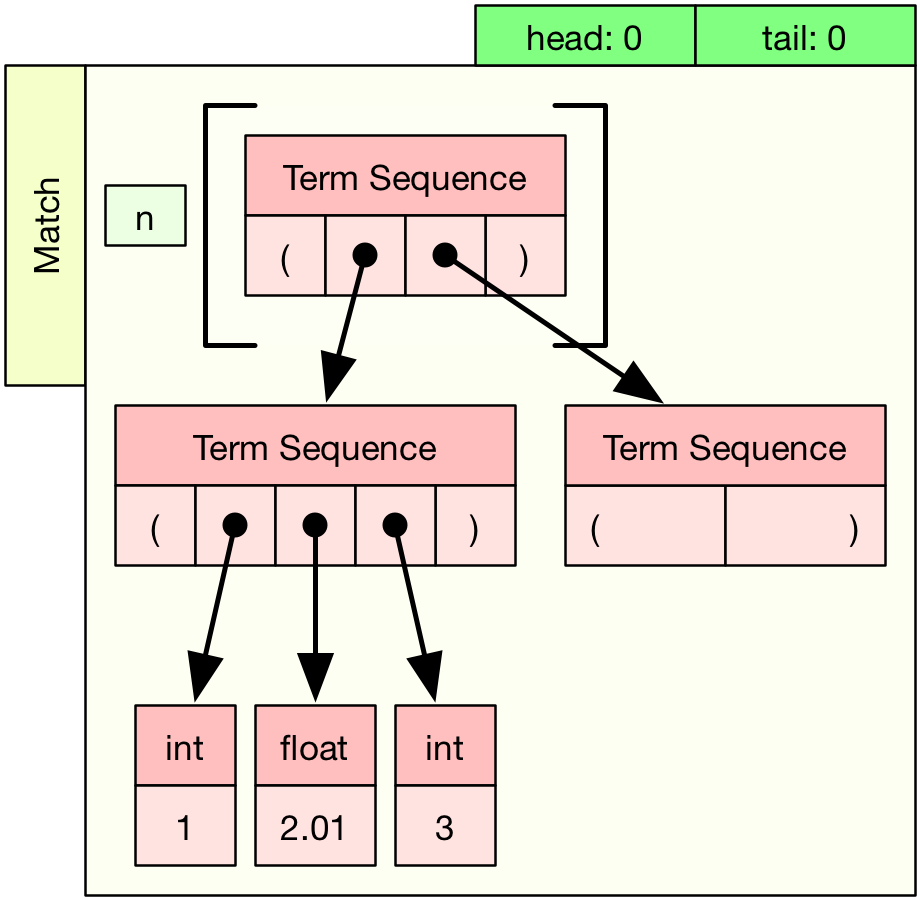
\includegraphics[scale=0.152]{ellipsis-example-matches-2.png}
\caption{Matches returned after matching term \texttt{()} against pattern \texttt{n ...}}
\label{ellipsis-example-matches-2}
\end{figure}

\begin{figure}[h]
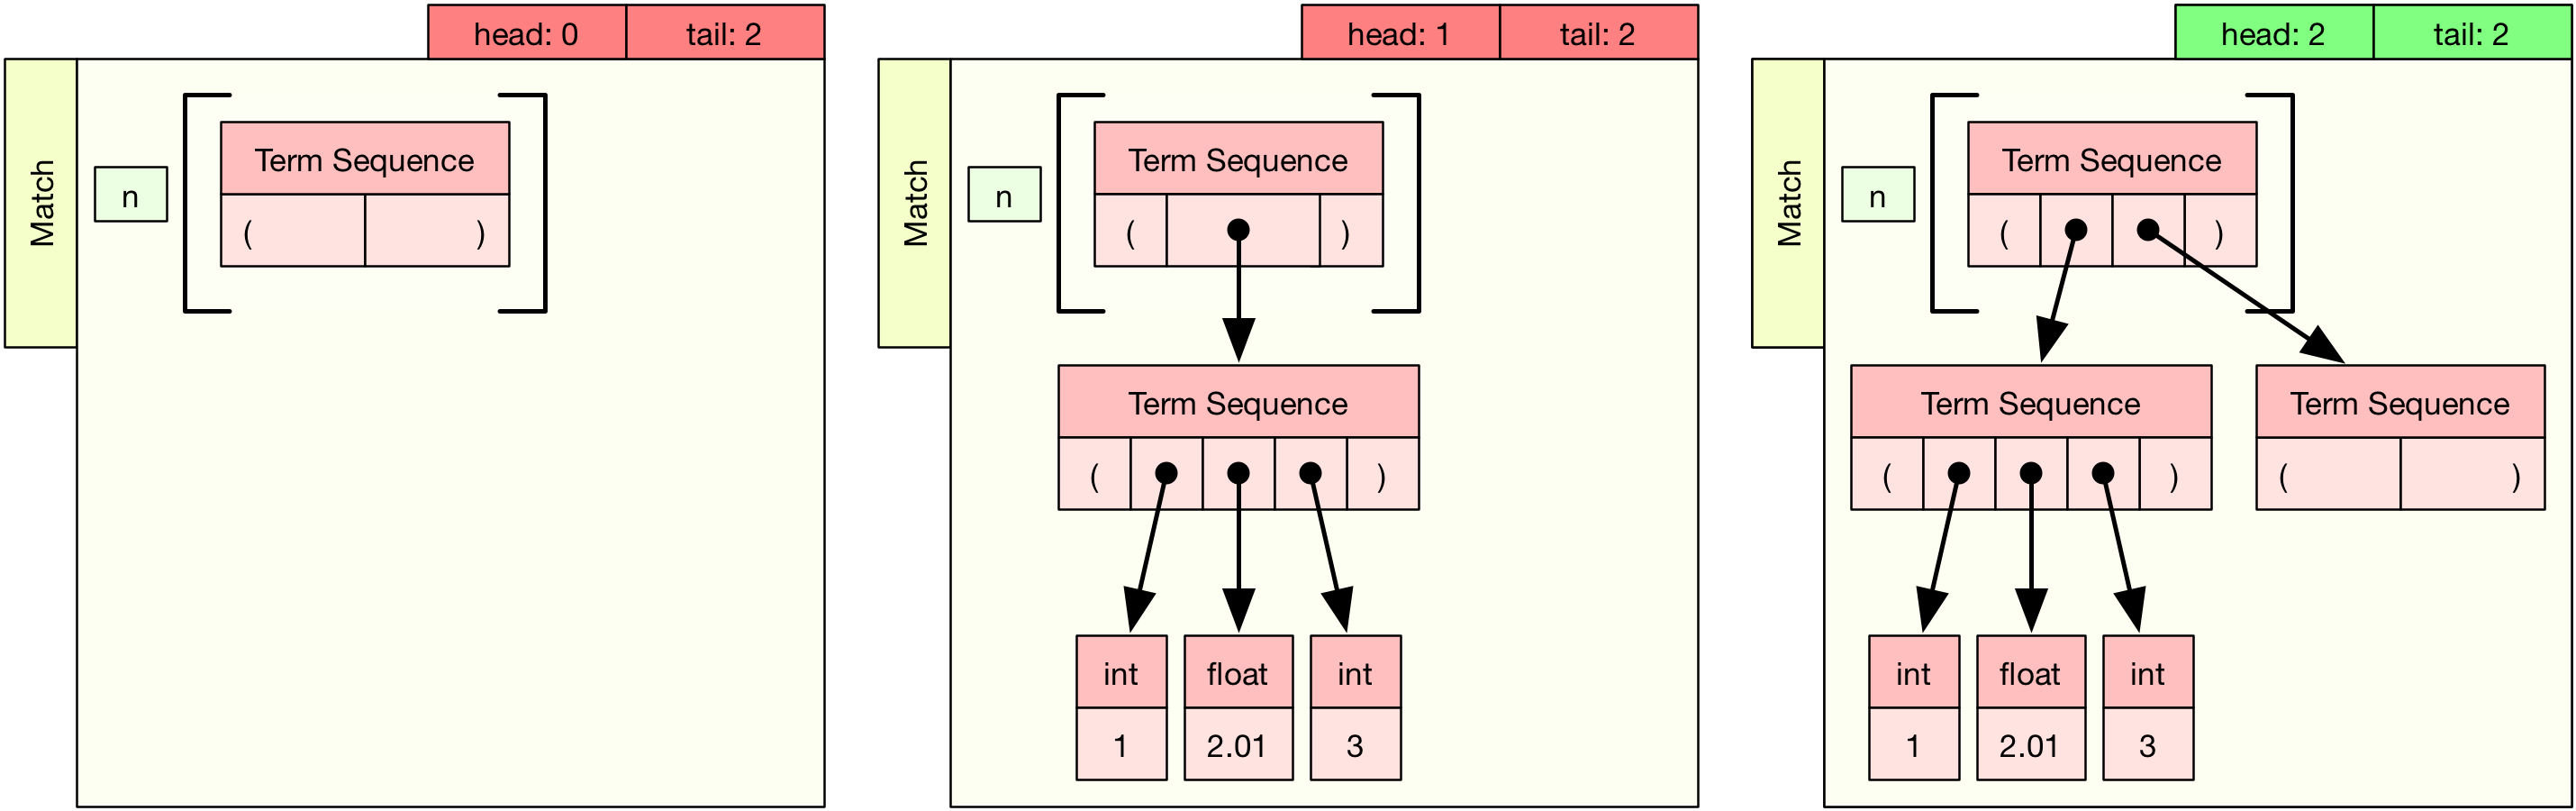
\includegraphics[scale=0.152]{ellipsis-example-matches-3.png}
\caption{Matches returned after matching term \texttt{((1 2 3)())} against pattern \texttt{(n ...) ...} }
\label{ellipsis-example-matches-3}
\end{figure}



\subsection{Match Function: InHole pattern}
Given pattern \InHolePattern, let $f_p^{impl}$ name of the function for \texttt{in-hole} pattern. Recall that \texttt{in-hole} pattern is annotated with pattern-variables during "Pattern Variable Extraction" pass described in Section TODO. Let $pv_i^{(p_1)}$ and $pv_i^{(p_2)}$ be annotations for $p_1$ and $p_2$. Finally, generate functions for $p_1$ and $p_2$ and let them be $f_{p_1}$ and $f_{p_2}$ respectively. 

Notice that this function contains extra parameter \texttt{path}, which is used to keep track of path to possible \texttt{hole}. To conform to established interface, a wrapper function will be generated later.

Since $p_1$ and $p_2$ are self-contained patterns with possible non-deterministic behaviour, \texttt{match} cannot be passed to $f_{p_1}$ and $f_{p_2}$ as is. Instead, create special \texttt{Match} instances to be passed to $f_{p_1}$ and $f_{p_2}$ that are initialized with $pv_i^{(p_1)}$ or $pv_i^{(p_2)}$ accordingly.

First, call $f_{p_2}$ with appropriate match, if resulting list of matches is non-empty, do the following: (1) append current term to the path; (2) call path copying function thus replacing the term with \texttt{hole} and (3) call $f_{p1}$ with appropriate match. If resulting set of matches is not empty, increment \texttt{head} (without overwriting it!) by one signalling successful matching of \texttt{in-hole} pattern, combine resulting matches of $f_{p_1}$ and $f_{p_2}$ with initial \texttt{match} as explained in Section TODO, and append to \texttt{matches}.

If given \texttt{term} is \texttt{Sequence}, continue matching \texttt{in-hole} pattern. Each element of the sequence is added to the path, $f_p^{impl}$ is called with said element, resulting matches are added to \texttt{matches} and topmost term in the \texttt{path} is popped. Resulting \texttt{matches} are returned.

%\setlength\LTleft{-65pt}% 2.5cm into the left margin
\begin{tabular}{|c|p{0.97\textwidth}|}
\hline 
\cellcolor{blue}1 & 
\begin{minted}[tabsize=1,obeytabs,escapeinside=||,mathescape=true,fontsize=\small]{python}
def codegenInHole(inhole):
	|$f_p^{impl}$| = symgen("match_pattern_impl")
	|$pv_1^{(p_1)}, ..., pv_n^{(p_1)}$| = |$p_1$|.getannotation(PatternVariables)
	|$pv_1^{(p_2)}, ..., pv_m^{(p_2)}$| = |$p_2$|.getannotation(PatternVariables)
	|$f_{p_1}, f_{p_2}$| = codegen(|$p_1$|), codegen(|$p_2$|)
\end{minted} 
\\
\hline 
\cellcolor{red}2 &
\begin{minted}[tabsize=1,obeytabs,escapeinside=||,mathescape=true,fontsize=\small]{python}
def |$f_p$|(term, match, head, tail, path):
	matches = []
	p2match = Match([|$pv_1^{(p_2)}, ..., pv_m^{(p_2)}$|])
	p2ms = |$f_{p_2}$|(term, p2match, 0, 1)
	if len(p2ms) != 0:
		p1match = Match(|$pv_1^{(p_1)}, ..., pv_n^{(p_1)}$|)
		npath = path + [term]
		nterm = copy_path_and_replace_last(tmp0, hole)
		p1ms = |$f_{p_1}$|(nterm, p1match, 0, 1)
		if len(p1ms) != 0:
			nhead = head + 1
			ms = match_cartesian_product_add_binding_to(
				p1ms, p2ms, match, nhead, tail)
			matches = matches + ms
\end{minted} 
\\
\hline
\cellcolor{green}3 & 
\begin{minted}[tabsize=1,obeytabs,escapeinside=||,mathescape=true,fontsize=\small]{python}
	if isinstance(term, Sequence):
		path.append(term)
		for i in range(term.length()):
			childterm = term.get(i)
			results= |$f_p^{impl}$|(childterm, match, 
								    head, tail, path)
			matches = matches + results 
		path.pop()
	 return matches 
\end{minted} 
\\
\hline
\end{tabular}

%\end{adjustwidth}

Finally, to get rid of \texttt{path} parameter from signature of $f_p^{impl}$, a wrapper function $f_p$ is generated. Additionally, it also handles constraint checks $c_i$ if applicable. Since constraint checks are optional, there are two cases to consider.

\begin{enumerate}
\item No constraint checks - simple return \texttt{matches}
\item Constraint checks are present - for each constraint check generate a call to \texttt{Match.comparekeys} function. This is done for each match returned by calling $f_p^{impl}$.
\end{enumerate}

\begin{minted}[tabsize=2,obeytabs,escapeinside=||,mathescape=true,fontsize=\small]{python}

def |$f_p$|(term, match, head, tail):
	matches = |$f_p^{impl}$|(match, head, tail, [])

	nmatches = []
	for m, h, t in matches:
	
	if not m.comparekeys(|$s_1$|, |$s_2$|):
		continue
	nmatches.append((m, h, t))
	
	return nmatches

	return matches

\end{minted} 

\subsection{Top-Level Matching Function}
Given some pattern $p$, generating top-level function for pattern involves the following steps: 

\begin{itemize}
\item Retrieve a set of pattern-variables $pv_1^{p}, ..., pv_n^{p}$ assigned in the pattern from annotation "PatternVariables".
\item Retrieve a set of pattern-variables $pvr_1^{p}, ..., pvr_m^{p}$ that are to be removed after matching from annotation "PatConstraintCheckRemoveVars" (see TODO section).
\item Let $f_p$ be the top-level function for pattern $p$.
\item Generate matching function $fm_p$ for pattern $p$.
\end{itemize}

Now, we get to code-generation. Initialize \texttt{Match} object with pattern-variables $pv_i^{p}$ and call $f_p$ with said \texttt{Match} instance, \texttt{head} and \texttt{tail} set to zero and one, respectively. After a list of matches is returned, need to strip out resulting \texttt{Match} from \texttt{(Match, int, int)}  tuples as well as remove symbols $pvr_i^{p}$ from \texttt{Match} instances. Resulting \texttt{Match} instances are appended to an array. Said array is then returned.


\begin{minted}[tabsize=2,obeytabs,escapeinside=||,mathescape=true,fontsize=\small]{python}

	
	
	
	
def $f_p$(term):
	match = Match(|$pv_1^{p}, ..., pv_n^{p}$|)
	matches = $fm_p$(term, match, 0, 1)
	ret = []	
	for m, h, t in matches:
	
		m.removekey(|$pvr_i^{p}$|}
		ret.append(m)
	
	return ret

\end{minted} 
